\documentclass[12pt,a4paper]{report}
\usepackage{graphicx}
\usepackage{amsmath}
\usepackage{fancyhdr}
\usepackage{cite}
\usepackage{framed}
\usepackage{float}
\usepackage{datetime2}
\usepackage{multicol}
%The below Section make chapter and its name to center of the page
\usepackage{blindtext}
\usepackage{xpatch}
\usepackage{geometry}
 \geometry{
 right=25mm,
 left=25mm,
 top=20mm,
 bottom=25mm,
 }
\usepackage{fontspec}
\usepackage{tocloft}

\usepackage{listings}
\usepackage{xcolor}
\usepackage{algorithm}
\usepackage{algorithmic}
\usepackage{hyperref}
\makeatletter
\renewcommand{\bibname}{References}
\renewcommand{\cftdot}{}
% \renewcommand{\cftchappresnum}{CHAPTER }
% \renewcommand{\cftchapaftersnum}{:}
% \renewcommand{\cftchapnumwidth}{6.5em}
% \renewcommand\cftfigindent{0pt}
% \renewcommand\cftfigpresnum{Figure\ }
% \renewcommand\cftfigaftersnum{ : }
% \renewcommand{\cftfignumwidth}{5.5em}
% \renewcommand{\cfttabpresnum}{Table\ }
% \renewcommand\cfttabaftersnum{ : }
% \renewcommand{\cfttabnumwidth}{5em}
\makeatother

% \renewcommand{\familydefault}{\sfdefault}


% Styles for Codes

\lstdefinestyle{htmlcssjs}{
    basicstyle=\ttfamily\footnotesize, % Code font and size
    numberstyle=\tiny\color{gray},     % Line number style
    numbers=left,                      % Line numbers on the left
    numbersep=5pt,                     % Line number spacing
    frame=single,                      % Frame around the code
    breaklines=true,                   % Line breaking
    tabsize=2,                         % Tab size
    showstringspaces=false,            % Don't show spaces
}

% HTML Style
\lstdefinelanguage{HTML}{
    language=html,
    sensitive=true,
    morecomment=[s]{<!--}{-->},
    morestring=[b]",
    tagstyle=\color{blue},
    stringstyle=\color{red},
    commentstyle=\color{green},
}

% CSS Style
\lstdefinelanguage{CSS}{
    language=css,
    sensitive=true,
    morecomment=[l]{//},
    morecomment=[s]{/*}{*/},
    morestring=[b]",
    keywordstyle=\color{purple},
    stringstyle=\color{red},
    commentstyle=\color{green},
}

% JavaScript Style
\lstdefinelanguage{JavaScript}{
    language=java,
    sensitive=true,
    morecomment=[l]{//},
    morecomment=[s]{/*}{*/},
    morestring=[b]",
    keywordstyle=\color{blue},
    stringstyle=\color{orange},
    commentstyle=\color{green},
}

% C++ Style
\lstdefinelanguage{CPP}{
    language=C++,
    morecomment=[l]{//},
    morecomment=[s]{/*}{*/},
    morestring=[b]",
    keywordstyle=\color{blue},
    stringstyle=\color{red},
    commentstyle=\color{green},
}



\makeatletter
\xpatchcmd{\@makeschapterhead}{%
  \Huge \bfseries  #1\par\nobreak%
}{%
  \Huge \bfseries\centering #1\par\nobreak%
}{\typeout{Patched makeschapterhead}}{\typeout{patching of @makeschapterhead failed}}


\xpatchcmd{\@makechapterhead}{%
  \huge\bfseries \@chapapp\space \thechapter
}{%
  \huge\bfseries\centering \@chapapp\space \thechapter
}{\typeout{Patched @makechapterhead}}{\typeout{Patching of @makechapterhead failed}}

\makeatother
%The above Section make chapter and its name to center of the page
%\unwanted packages also included
\linespread{1.5}
% \pagestyle{fancy}
% \fancyhead{}
% %\header and footer section
% \renewcommand\headrulewidth{0.1pt}
% \fancyhead[L]{\footnotesize \leftmark}
% \fancyhead[R]{\footnotesize \thepage}
% \renewcommand\headrulewidth{0pt}
% % \fancyfoot[R]{\small RANAGHAT GOVERNMENT POLYTECHNIC}
% \renewcommand\footrulewidth{0.1pt}
% \fancyfoot[C]{2024 - 2025}
% \fancyfoot[L]{\small Single lead mobile ECG machine}




\begin{document}

\begin{center}
{\Large \textbf{Single lead mobile ECG machine}}\\
\vspace{0.5cm}

A PROJECT REPORT\\
SUBMITTED IN PARTIAL FULFILLMENT OF THE REQUIREMENTS\\
FOR THE AWARD OF THE DIPLOMA\\
IN\\
\textbf{Electical Engineering} \\
\vspace{1 cm}
Submitted by: \\

% \begin{multicols}{3}
% \vspace{1cm}
SUDIPTA SEN(D222322587)\\
\vspace{0.2cm}

% \vspace{1cm}
TANIMA GHOSH(D222322596)\\
\vspace{0.2cm}

% \vspace{1cm}
RAJU ADHIKARY(D222322568)\\
\vspace{0.2cm}

% \vspace{1cm}
GOUTAM AMBALI(D202116553)\\
\vspace{0.2cm}

% \vspace{1cm}
RUMA MANDI(D222322574)\\
\vspace{0.2cm}
% \end{multicols}
\vspace{1 cm}
Under the guidance of\\

Lec.(Mr.) SOUVIK BAG\\

\end{center}

% \vspace{4pt}
\begin{center}
\begin{figure}[H]
    \centering
    
\includegraphics[scale=0.1]{images/institute_logo.png}
    \label{fig:institute_logo}
\end{figure}
\textbf{DEPT. OF ELECTRICAL ENGINEERING}\\

RANAGHAT GOVERNMENT POLYTECHNIC\\

Ranaghat, Nadia-741201 \\
\textbf{DEC 2024}\\
\end{center}

\thispagestyle{empty}

\newpage



\newpage

\pagenumbering{roman}

%\Declaration in this page.


\begin{center}


\begin{center}
%\vspace{1.5cm}
\textbf{DEPT. OF ELECTRICAL ENGINEERING}\\

RANAGHAT GOVERNMENT POLYTECHNIC \\

Ranaghat, Nadia-741201\\
\end{center}
\vspace{2 cm}
\textbf{\underline{CANDIDATE’S DECLARATION}}\\
\addcontentsline{toc}{chapter}{Candidate’s Declaration}
\end{center}
\vspace{1.2cm}
We, SUDIPTA SEN (D222322587), TANIMA GHOSH (D222322596), RAJU ADHIKARY (D222322568), GOUTAM AMBALI (D202116553) \& RUMA MANDI (D222322574) students of Diploma (ELECTRICAL ENGINEERING), hereby declare that the Project Dissertation titled -- “Single lead mobile ECG machine” which is submitted by us to the Department of Electical Engineering, RANAGHAT GOVERNMENT POLYTECHNIC, West Bengal in fulfillment of the requirement for awarding of Diploma, is not copied from any source without proper citation. This work has not previously formed the basis for the award of any Diploma or other similar title or recognition in our institute.


% \begin{description}
%   \item [Title of the Paper] Identification of IUU Transshipment Activity Using AIS Data.
%   \item[Author names] Harshit Muhal, Ishan Chaudhary, Kirti Dabas 
%   \item[Name of Conference/Journal] International Conference for Emerging Technology 2022
%   \item [Conference Dates with the venue (if applicable)]Online (27-29 May 2022)
%   \item [Have you registered for the conference (Yes/No)?] Yes
%   \item [Status of paper (Accepted/Published/Communicated)] Accepted
%   \item [Date of paper acceptance] 02 FEBRUARY 2022
%   \item [Date of paper publication] YET TO BE PUBLISHED
% \end{description}

\noindent \begin{minipage}{3.6cm}
\begin{flushleft}
\vspace{5 cm}
                         
Place: West Bengal\\
Date: 2024-12-11\\

\end{flushleft} 
\end{minipage}
\hfill
\begin{minipage}{13.6cm}
\begin{flushright}                                      
\vspace{5 cm}
\begin{multicols}{3}
\textbf{SUDIPTA SEN}
\textbf{(D222322587)}\\
\vspace{0.2cm}

\textbf{TANIMA GHOSH}
\textbf{(D222322596)}\\
\vspace{0.2cm}

\textbf{RAJU ADHIKARY}
\textbf{(D222322568)}\\
\vspace{0.2cm}

\textbf{GOUTAM AMBALI}
\textbf{(D202116553)}\\
\vspace{0.2cm}

\textbf{RUMA MANDI}
\textbf{(D222322574)}\\
\vspace{0.2cm}
\end{multicols}


\end{flushright} 
\end{minipage}

\thispagestyle{empty}

\newpage


\begin{center}
%\vspace{1.5cm}
\textbf{DEPT. OF ELECTRICAL ENGINEERING}\\

RANAGHAT GOVERNMENT POLYTECHNIC \\

Ranaghat, Nadia-741201\\
\end{center}

\vspace{2cm}
\begin{center}
 \textbf{\underline {CERTIFICATE}}
 \addcontentsline{toc}{chapter}{Certificate}
\end{center}
\sloppy I hereby certify that the Project titled "Single lead mobile ECG machine” which is submitted by SUDIPTA SEN (D222322587), TANIMA GHOSH (D222322596), RAJU ADHIKARY (D222322568), GOUTAM AMBALI (D202116553) \& RUMA MANDI (D222322574) for fulfillment of the requirements for awarding of the Diploma is a record of the project work carried out by the students under my guidance \& supervision. To the best of my knowledge, this work has not been submitted in any part or fulfillment for any Degree or Diploma to this Institute or elsewhere.

\noindent \begin{minipage}{4cm}
\begin{flushleft}
\vspace{1 cm}
                         
Place : West Bengal \\
Date : 2024-12-11 \\

\end{flushleft} 
\end{minipage}
\hfill
\begin{minipage}{10cm}
\begin{flushright}                                      
\vspace{2cm}
                         

\vspace{.8cm}
\textbf{Lec.(Mr.) SOUVIK BAG}\\
\textbf{(SUPERVISOR)}\\
Lecturer\\
Department of ELECTRICAL ENGINEERING \\
RANAGHAT GOVERNMENT POLYTECHNIC\\
\end{flushright} 
\end{minipage}
% \thispagestyle{empty}

\newpage
% Please remove and edit percentage(%) Symbol, if you want this Acknowledgement page in your report. As per ktu guideline, this page is not necessary. 

% \begin{abstract}

\begin{center}
 \textbf{ABSTRACT}
 \addcontentsline{toc}{chapter}{Abstract}
\end{center}

\textbf{Keywords} - Portable ECG, Low-Cost Healthcare Technology, Rural Health Diagnostics

\vspace{0.8cm}

This project presents a cost-effective, portable, single-lead ECG (Electrocardiogram) machine designed to meet essential cardiac monitoring needs, particularly in underserved rural or remote areas. Multi-lead ECG machines are often costly and complex, limiting accessibility and usability in such settings. Our single-lead ECG device focuses on affordability, ease of use, and mobility without compromising essential diagnostic functionality.

The proposed system leverages bioinstrumentation amplifiers, precision filters, and a DIY digital storage oscilloscope (DSO) to capture, amplify, and visualize ECG signals. Using Wi-Fi-enabled technology, this prototype also supports data transfer and remote monitoring capabilities. Through systematic design and practical implementation, this project successfully demonstrates real-time ECG signal processing with a user-friendly interface.

In future iterations, we aim to integrate AI-driven health analytics, enhanced wireless capabilities, and expanded outreach for rural healthcare initiatives. This project underscores the potential of affordable healthcare technology to improve access to vital diagnostic tools, addressing a critical gap in global health equity.
%  \end{abstract} 

\newpage
\addcontentsline{toc}{chapter}{Acknowledgement}

\chapter*{\centering \large ACKNOWLEDGEMENT\markboth{Acknowledgements}{Acknowledgements}}

The successful completion of any task is incomplete and meaningless without giving any due credit to the people who made it possible without which the project would not have been successful and would have existed in theory.

First and foremost, we are grateful to \textbf{Mr. Achanchal Kundu}, HOD, Department of Electical Engineering, RANAGHAT GOVERNMENT POLYTECHNIC, and all other faculty members of our department for their constant guidance and support, constant motivation and sincere support and gratitude for this project work. We owe a lot of thanks to our supervisor, \textbf{Mr. Souvik Bag}, Lecturer, Department of Electical Engineering, RANAGHAT GOVERNMENT POLYTECHNIC for igniting and constantly motivating us and guiding us in the idea of a creatively and amazingly performed Major Project in undertaking this endeavor and challenge and also for being there whenever we needed his guidance or assistance.


We would also like to take this moment to show our thanks and gratitude to one and all, who indirectly or directly have given us their hand in this challenging task. We feel happy and joyful and content in expressing our vote of thanks to all those who have helped us and guided us in presenting this project work for our Major project. Last, but never least, we thank our well-wishers and parents for always being with us, in every sense and constantly supporting us in every possible sense whenever possible.



\vspace{1 cm}                        
\begin{multicols}{3}
\centering
\textbf{SUDIPTA SEN}
\textbf{(D222322587)}\\
\vspace{0.3cm}


\textbf{TANIMA GHOSH}
\textbf{(D222322596)}\\
\vspace{0.3cm}


\textbf{RAJU ADHIKARY}
\textbf{(D222322568)}\\
\vspace{0.3cm}


\textbf{GOUTAM AMBALI}
\textbf{(D202116553)}\\
\vspace{0.3cm}
\sloppy

\textbf{RUMA MANDI}
\textbf{(D222322574)}\\
\vspace{0.3cm}
\end{multicols}

\tableofcontents %This command used for index.
% \newpage
% \listoftables

\addcontentsline{toc}{chapter}{List of Figures}

% \newpage
\listoffigures
% \addcontentsline{toc}{chapter}{List of Tables}



\newpage

\begin{center}
  \textbf{LIST OF SYMBOLS, ABBREVIATIONS AND NOMENCLATURE} 
\end{center}
\addcontentsline{toc}{chapter}{List of Symbols, Abbreviations}

\begin{itemize}
  \item[] \textbf{ECG}  : Electrocardiogram
  \item[] \textbf{EEG}  : Electroencephalogram
  \item[] \textbf{CVDs} : Cardiovascular Diseases
  \item[] \textbf{DIY}  : Do It Yourself
  \item[] \textbf{AD8232} : Bioinstrumentation Amplifier
  \item[] \textbf{DSO}  : Digital Storage Oscilloscope
  \item[] \textbf{MCU}  : Microcontroller Unit
  \item[] \textbf{Wi-Fi} : Wireless Fidelity
  \item[] \textbf{HTTP} : Hypertext Transfer Protocol
  \item[] \textbf{UI}   : User Interface
  \item[] \textbf{API}  : Application Programming Interface
  \item[] \textbf{ESP8266} : Wi-Fi Module
  \item[] \textbf{RC Filter} : Resistor-Capacitor Filter
  \item[] \textbf{DNS}  : Domain Name System
  \item[] \textbf{IoT}  : Internet of Things
\end{itemize}

\vspace{0.5cm}

\begin{center}
  \textbf{Technical Terms and Concepts} 
\end{center}

\begin{itemize}
  \item[] \textbf{Bioinstrumentation} : Application of electronics and measurement techniques for physiological data.
  \item[] \textbf{Signal Amplification} : Increasing the amplitude of ECG signals.
  \item[] \textbf{Baseline Wander} : Low-frequency noise caused by body movements or respiration.
  \item[] \textbf{Electromagnetic Interference (EMI)} : Disturbances from external electromagnetic sources.
  \item[] \textbf{WebSocket Protocol} : Real-time full-duplex communication channel.
  \item[] \textbf{Telemedicine} : Technology-based remote medical diagnostics and monitoring.
  \item[] \textbf{Graphical User Interface (GUI)} : Visual interface for user interaction.
  \item[] \textbf{Sinoatrial Node} : The natural pacemaker of the heart.
  \item[] \textbf{Real-Time Visualization} : Instant display of ECG signals for analysis.
  \item[] \textbf{Motion Artifacts} : Signal distortions caused by physical movements.
\end{itemize}

\vspace{0.5cm}

\begin{center}
  \textbf{Design Elements} 
\end{center}

\begin{itemize}
  \item[] \textbf{Spiral Copper Electrodes} : Custom reusable electrodes for ECG acquisition.
  \item[] \textbf{Low-Cost Healthcare Technology} : Affordable solutions for underserved areas.
  \item[] \textbf{Noise Filtering} : Removing unwanted signals from ECG data.
  \item[] \textbf{Single-Lead ECG} : Measuring electrical activity from one point on the body.
  \item[] \textbf{Precision Filters} : High-pass and low-pass filters for signal processing.
  \item[] \textbf{Wireless Data Transmission} : Sending ECG data via Wi-Fi.
  \item[] \textbf{Voltage Per Division (Volt/Div)} : Scaling unit for voltage on an oscilloscope.
  \item[] \textbf{Time Per Division (Time/Div)} : Scaling unit for time on an oscilloscope.
\end{itemize}

\vspace{0.5cm}

\begin{center}
  \textbf{Advanced and Future Concepts} 
\end{center}

\begin{itemize}
  \item[] \textbf{AI-Driven Analytics} : Artificial Intelligence for automated diagnostics.
  \item[] \textbf{Health Equity} : Ensuring equal access to medical resources.
  \item[] \textbf{Signal Processing} : Techniques for improving signal quality.
  \item[] \textbf{Remote Monitoring} : Analyzing health data from a distance.
  \item[] \textbf{Data Visualization Algorithms} : Computational methods for graphical data display.
\end{itemize}


% \thispagestyle{empty}


\newpage

\pagenumbering{arabic}    

\chapter{Introduction}
In today’s world, cardiovascular diseases (CVDs) are one of the leading causes of mortality, claiming millions of lives every year. Early detection and timely monitoring of heart health are crucial for managing these conditions effectively. However, in many rural and remote areas, access to advanced healthcare facilities is limited, leaving a significant portion of the population at risk of undiagnosed heart conditions. 

Imagine a scenario: A middle-aged farmer working in a rural area experiences occasional chest discomfort but dismisses it due to lack of access to medical facilities. One day, he suffers a major heart event because his condition went undetected for years. This is not just an isolated case but a recurring reality in underserved regions. What if there was a device that could have detected his heart condition earlier, allowing timely intervention?  

Electrocardiography (ECG) is an indispensable tool for diagnosing cardiac conditions by analyzing the heart's electrical activity. However, conventional ECG systems—often multi-lead, hospital-grade machines—pose barriers in rural and low-resource settings due to high costs, bulkiness, and the requirement for trained personnel.

Our project - \textbf{Micro-ECG} aims to eliminate these limitations by offering a fully portable, battery-powered, single-lead ECG system that uses:
\begin{itemize}
    \item A WiFi-based microcontroller (ESP8266) for communication.
    \item A real-time, browser-based user interface via captive portal.
    \item Hardware-level noise suppression using op-amps and RC filters.
    \item Frontend ECG signal filtering using hand-crafted JavaScript code.
\end{itemize}

Unlike Bluetooth-based systems or mobile apps, Micro-ECG works independently across devices, requiring only a browser to operate. With both on-device and external chest electrodes, it captures and visualizes cardiac signals accurately.






\chapter{Background}
The heart generates electrical impulses via the sinoatrial (SA) node, which propagate through the atria, AV node, and ventricles. This electrical conduction results in waveform patterns—P wave, QRS complex, and T wave—which an ECG captures.

\begin{figure}[H]
    \centering
    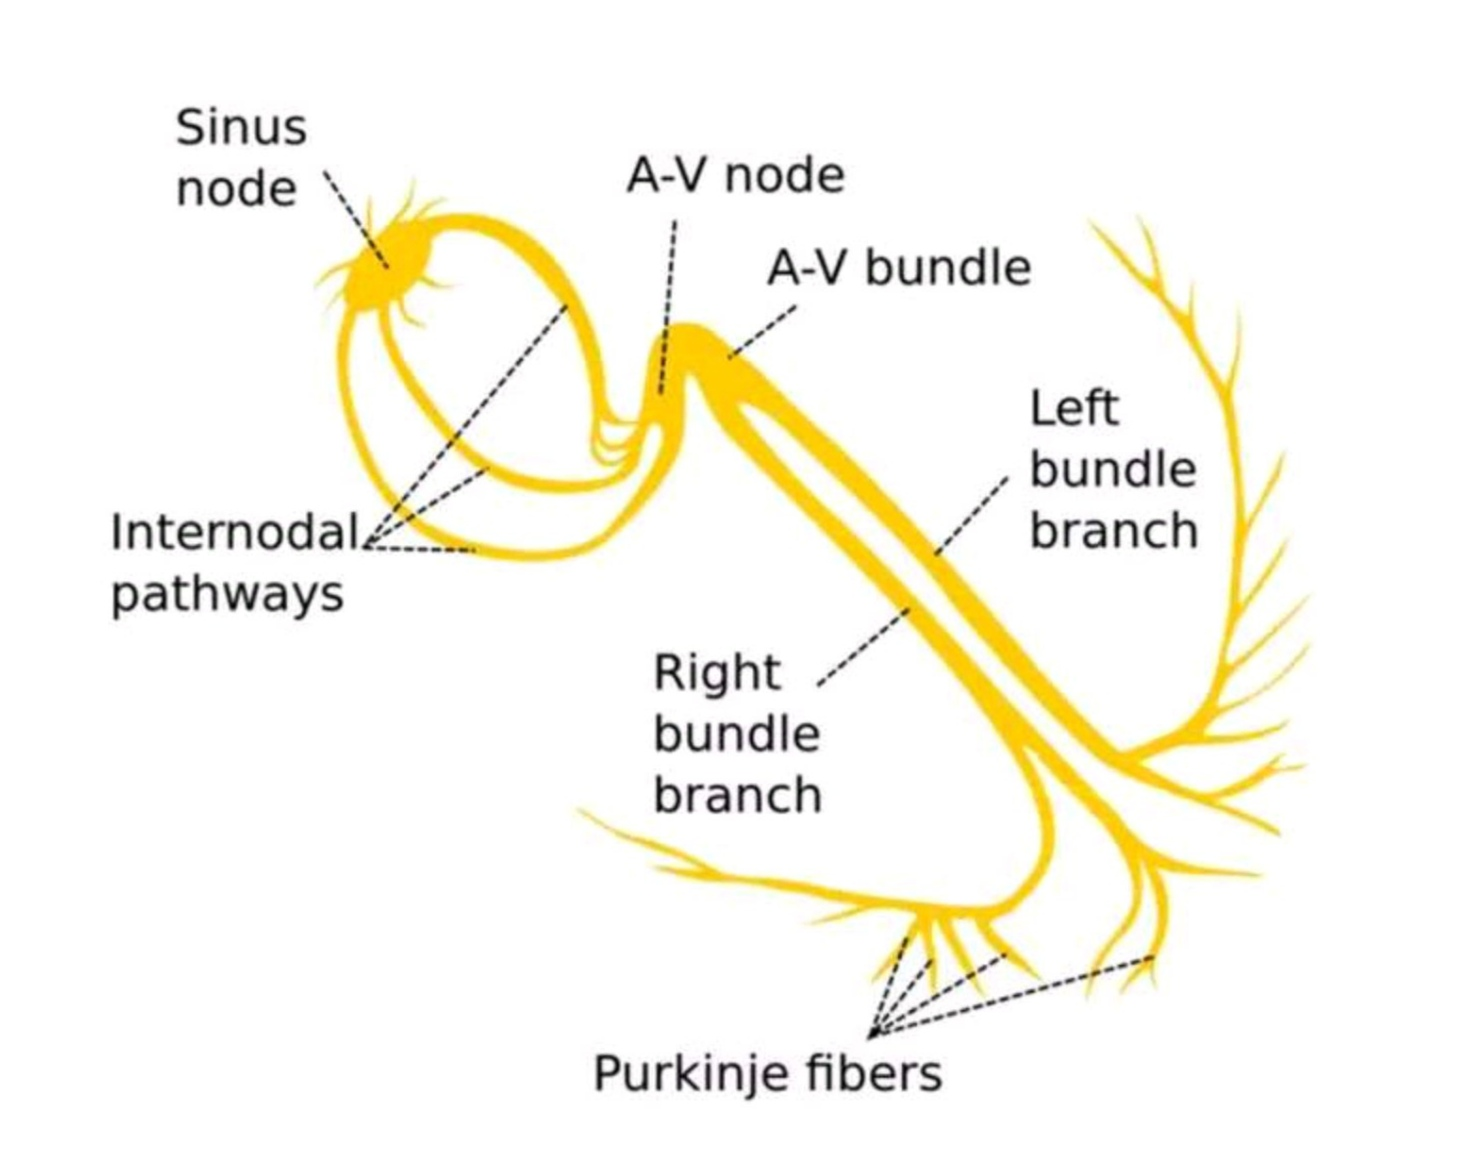
\includegraphics[width=0.7\textwidth]{images/electrical_heart.jpg}
    \caption{The electrical conduction system of the heart}
    \label{fig:electrical_heart}
\end{figure}

\begin{figure}[H]
    \centering
    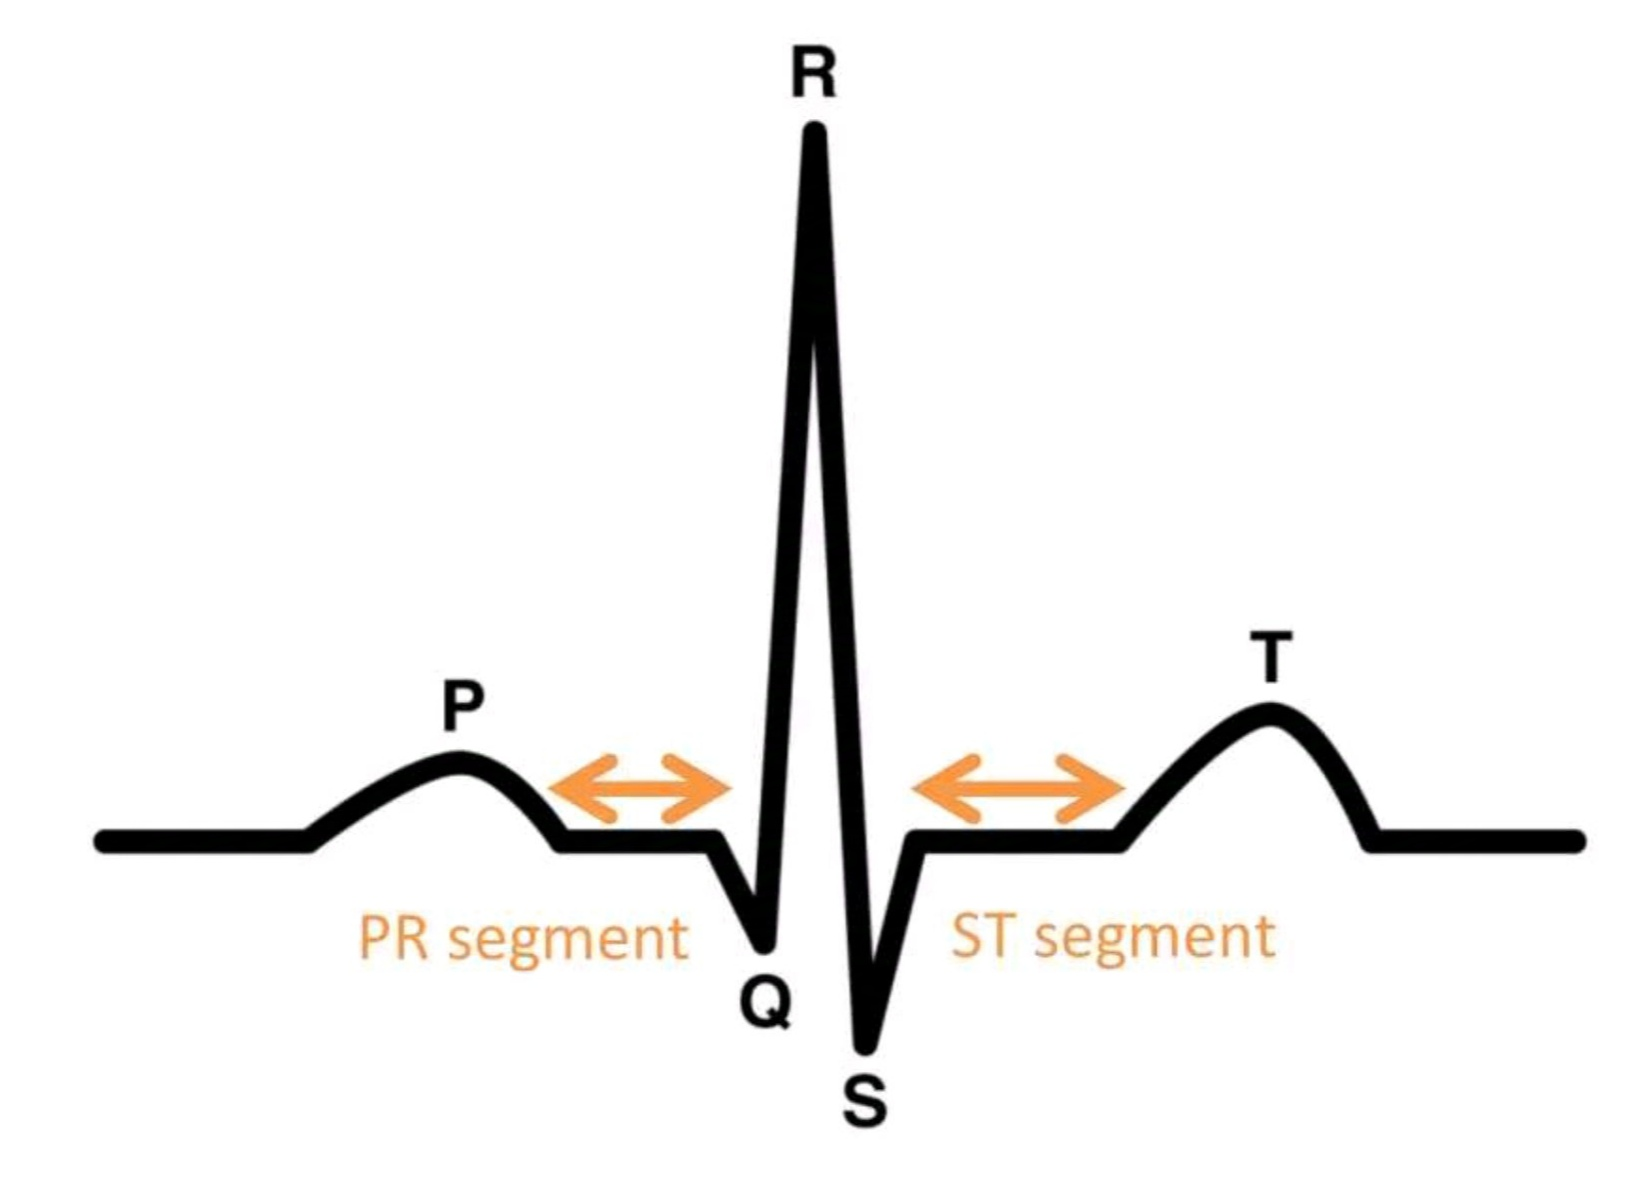
\includegraphics[width=0.7\textwidth]{images/pqrst.jpg}
    \caption{Normal ECG signal pattern with signal points}
    \label{fig:pqrst}
\end{figure}

Traditional 12-lead ECG machines provide comprehensive cardiac information but:
\begin{itemize}
    \item Are expensive (INR 20,000+).
    \item Require hospital-grade calibration.
    \item Depend on skilled interpretation.
\end{itemize}

\begin{figure}[H]
    \centering
    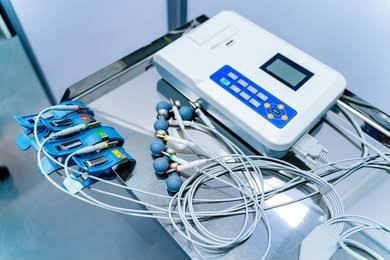
\includegraphics[width=0.7\textwidth]{images/hospital_ecg.jpg}
    \caption{Traditional Hospital ECG Machine}
    \label{fig:hospital_ecg}
\end{figure}

For early detection, especially of rhythm abnormalities like bradycardia or tachycardia, a single-lead solution is sufficient. This makes the single-lead ECG valuable for first-line screening, community health workers, and telemedicine.







\chapter{System Architecture}

\section{Block-Level Architecture}
The device consists of the following major subsystems:
\begin{enumerate}
    \item \textbf{Electrode Interface:} Captures surface potential using LA/RA finger contacts or optional chest leads.
    \item \textbf{Analog Front-End:} Uses AD8232 IC with discrete RC filter stages to suppress motion noise and 50Hz interference.
    \item \textbf{Microcontroller Unit:} ESP8266 with 10-bit ADC, serving both the UI and WebSocket data stream.
    \item \textbf{UI System:} Hosted from internal flash, drawn on HTML5 canvas, processes incoming ADC samples.
    \item \textbf{Battery and Power Management:} A 1200mAh Li-ion battery powers all modules with a Micro-USB port limited to charging and flashing.
\end{enumerate}

\begin{figure}[H]
    \centering
    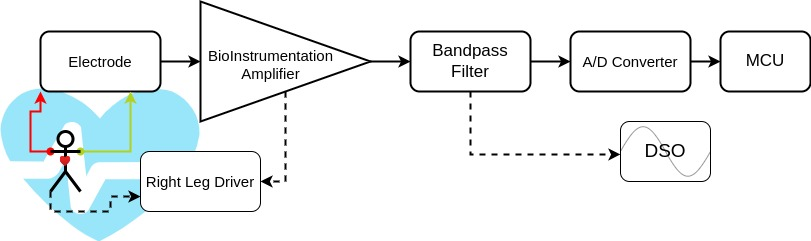
\includegraphics[width=0.8\textwidth]{images/ecg_block_diagram.jpg}
    \caption{ECG block diagram}
    \label{fig:ecg_block_diagram}
\end{figure}

\section{Data Flow Overview}
The ECG signal path is as follows:
\begin{itemize}
    \item \textbf{Step 1:} Electrical signal picked up via skin contact.
    \item \textbf{Step 2:} Passed to AD8232, which filters, amplifies, and outputs analog ECG signal.
    \item \textbf{Step 3:} ESP8266 samples the analog ECG at 200–500Hz.
    \item \textbf{Step 4:} Packets of ADC values are streamed via WebSocket.
    \item \textbf{Step 5:} HTML+JS frontend buffers and renders the waveform in real time.
\end{itemize}

\begin{figure}[H]
    \centering
    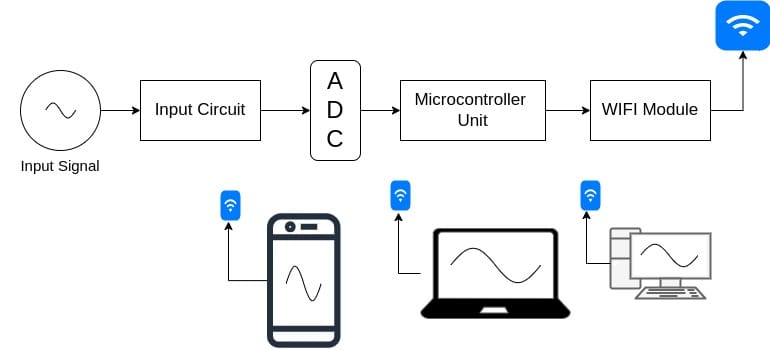
\includegraphics[width=0.7\textwidth]{images/dso_block_diagram.jpg}
    \caption{Analog to Digital Signal flow  block diagram}
    \label{fig:dso_block_diagram}
\end{figure}

\section{Key Features}
\begin{itemize}
    \item Real-time visualization via any browser without app installation.
    \item WebSocket-based data delivery ensures low latency.
    \item Captive portal works even without internet.
    \item Chest lead option increases signal fidelity.
    \item Lightweight filtering on hardware and software layers.
\end{itemize}






\chapter{Hardware Design}

\begin{figure}[H]
    \centering
    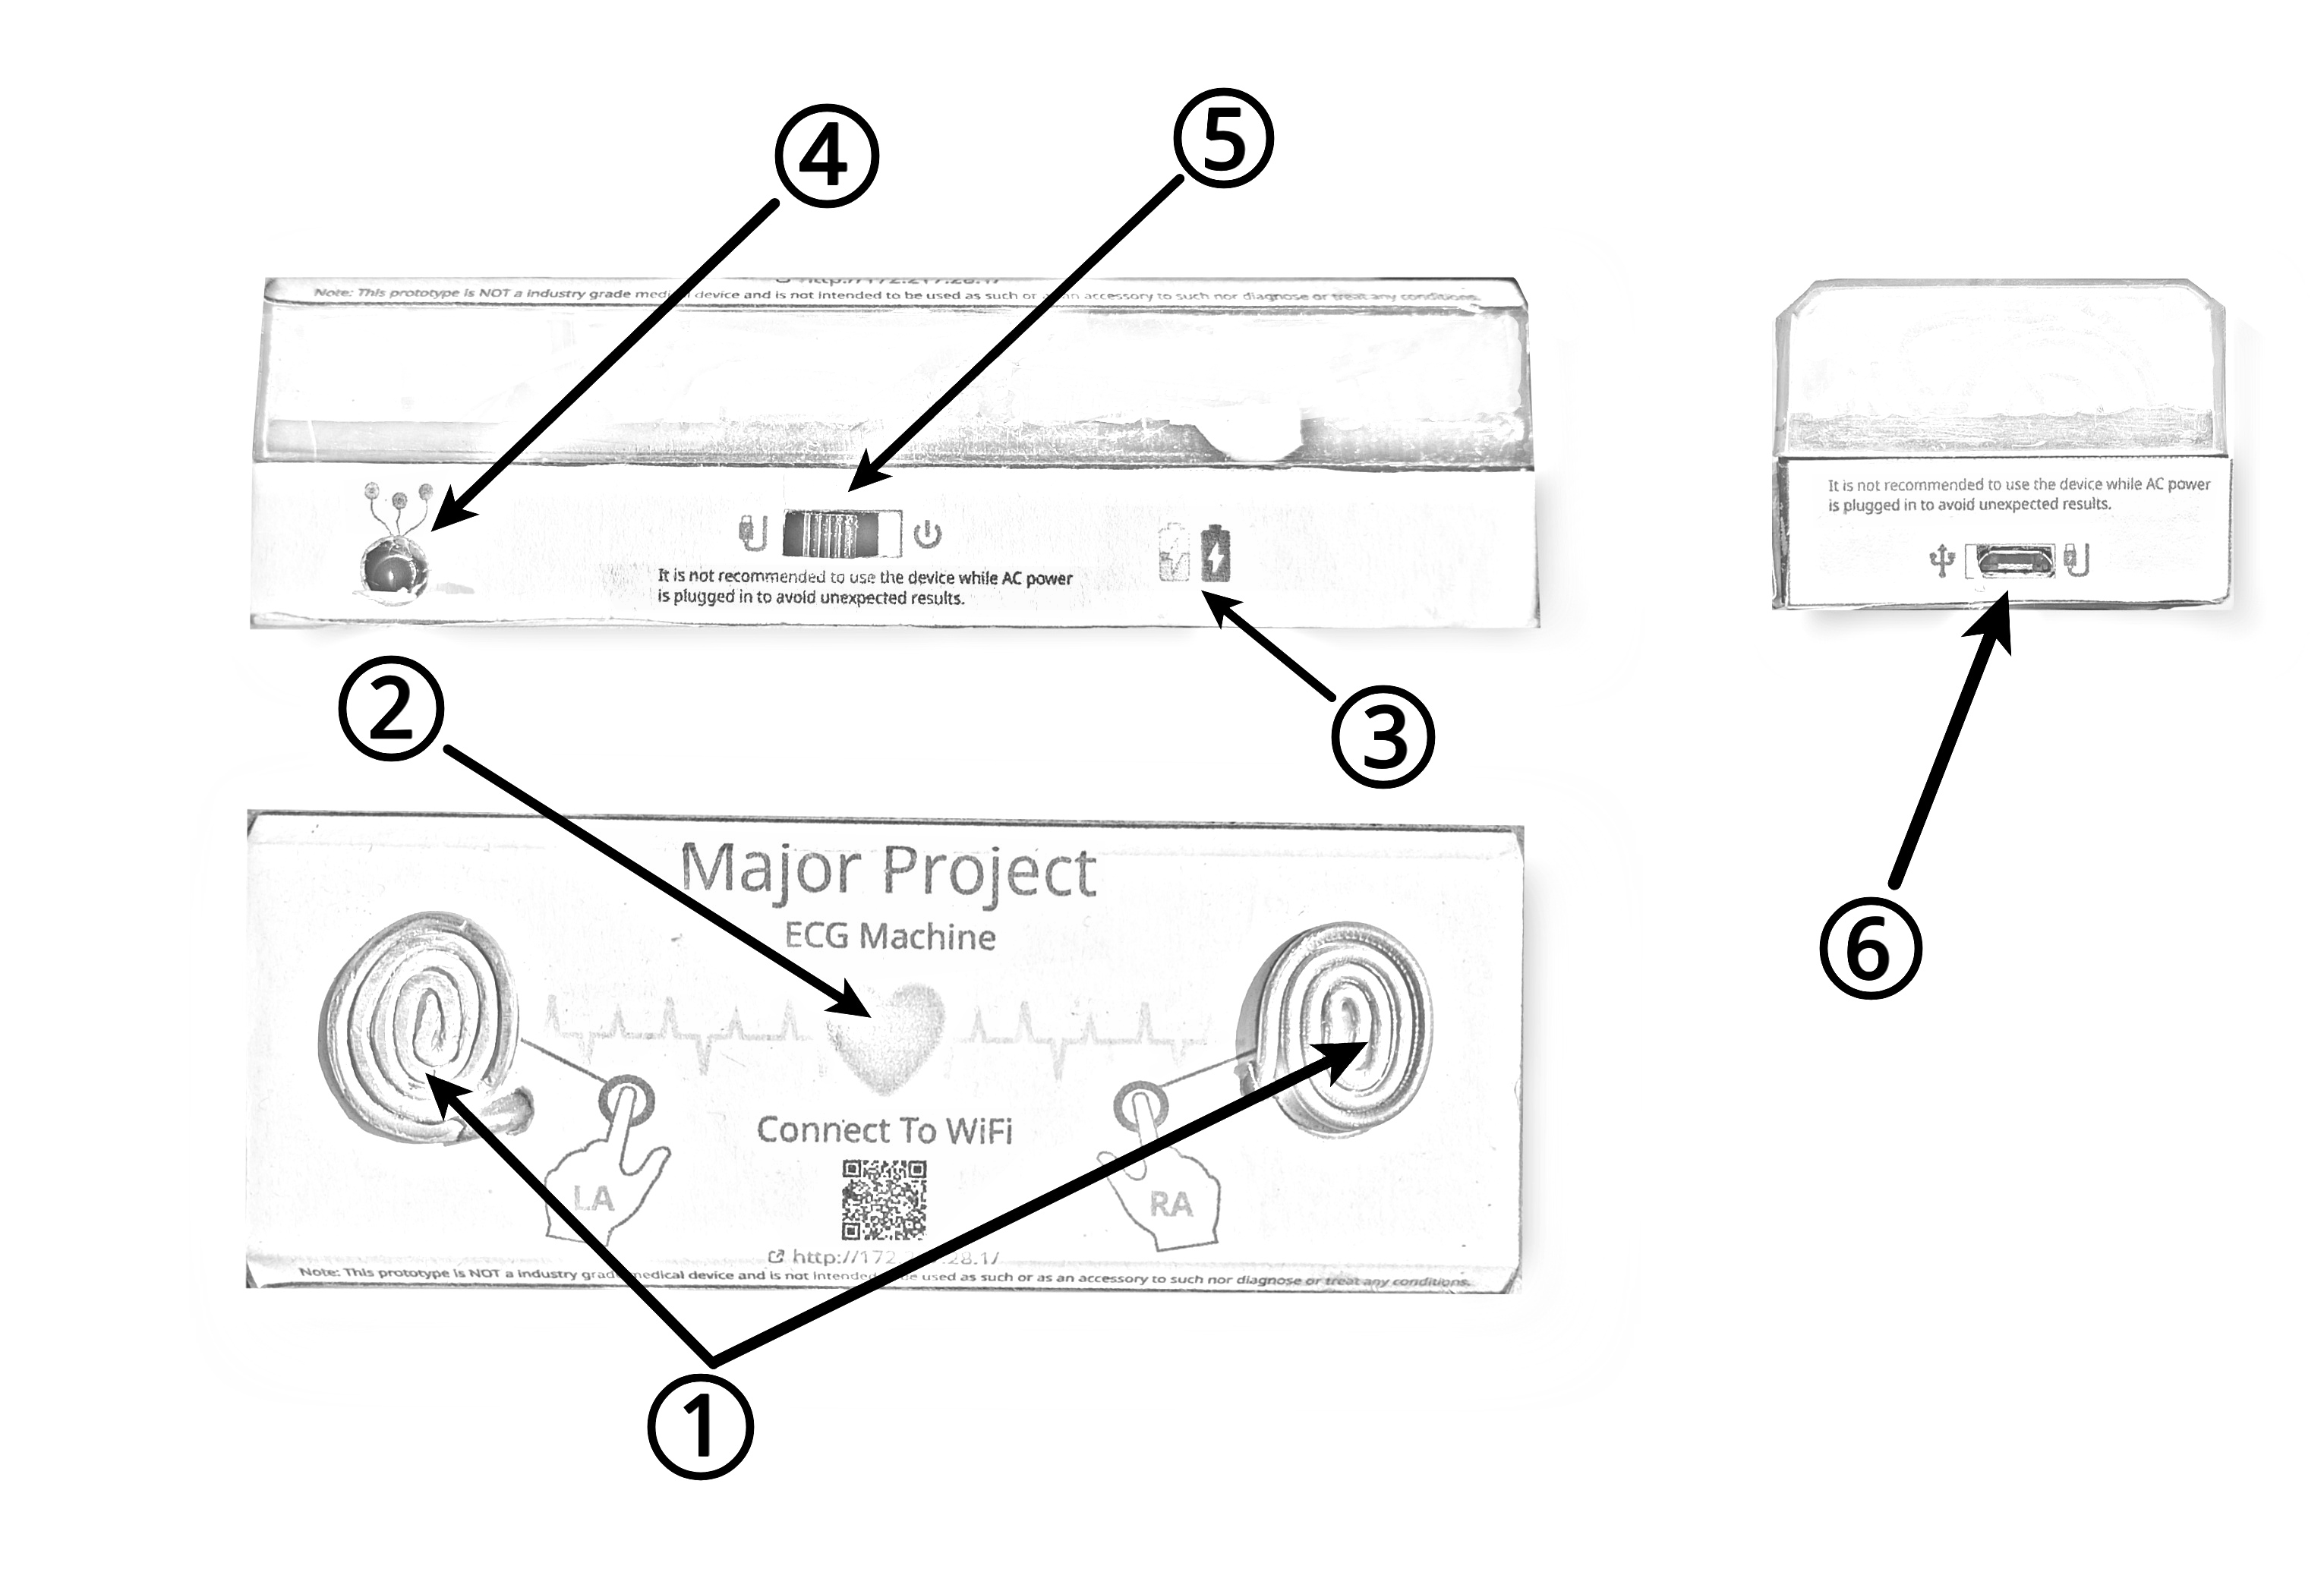
\includegraphics[width=0.7\textwidth]{images/proto_overview.png}
    \caption{Prototype Overview}
    \label{fig:proto_overview}
\end{figure}
{\small
\begin{enumerate}
    \item \textbf{LA \& RA Electrodes (Touch Type):} Finger placement electrodes for Left Arm (LA) and Right Arm (RA) detection. These are the primary contact points for quick ECG readings.
    \item \textbf{Heart LED Indicator:} Blinks in sync with the detected heart rhythm. Also shows device power status.
    \item \textbf{Charging Status LED:} \\ \textcolor{red}{Red} – Charging,\\ \textcolor{blue}{Blue} – Fully charged.
    \item \textbf{External Electrode Port:} Alternative electrode input, typically for chest placement using gel electrodes for improved accuracy.
    \item \textbf{Slide Switch (Charge-Off-On):} \\ \textit{Charge} – Enables charging without powering on the device.\\ \textit{Off} – Completely powered off.\\ \textit{On} – Powers the device for use.
    \item \textbf{Micro-USB Port:} Used for charging and firmware updates only. \\ \textbf{Note:} Do not use the device while charging to avoid inaccurate results.
\end{enumerate}
}
\section{Electrodes}
Micro-ECG provides two types of electrode input:
\begin{itemize}
    \item \textbf{Integrated Electrodes (Top):} LA and RA contacts on the top surface for direct finger placement. Fingerpads are made of copper wire, ensuring good skin contact. Wider surface contact improves signal quality.
    \item \textbf{External Chest Electrode Port:} A front-facing 3.5mm port allows optional chest-mounted electrode placement. This method provides higher signal amplitude and better baseline stability due to reduced motion artifacts.
\end{itemize}

\section{Analog Front-End Circuitry}
At the core is the \textbf{AD8232} AFE (Analog Front-End), chosen for its compact ECG functionality. The IC includes:
\begin{itemize}
    \item Instrumentation amplifier with high CMRR.
    \item Adjustable gain using external resistor ($G = 1 + \frac{100k\Omega}{R_G}$).
    \begin{figure}[H]
    \centering
        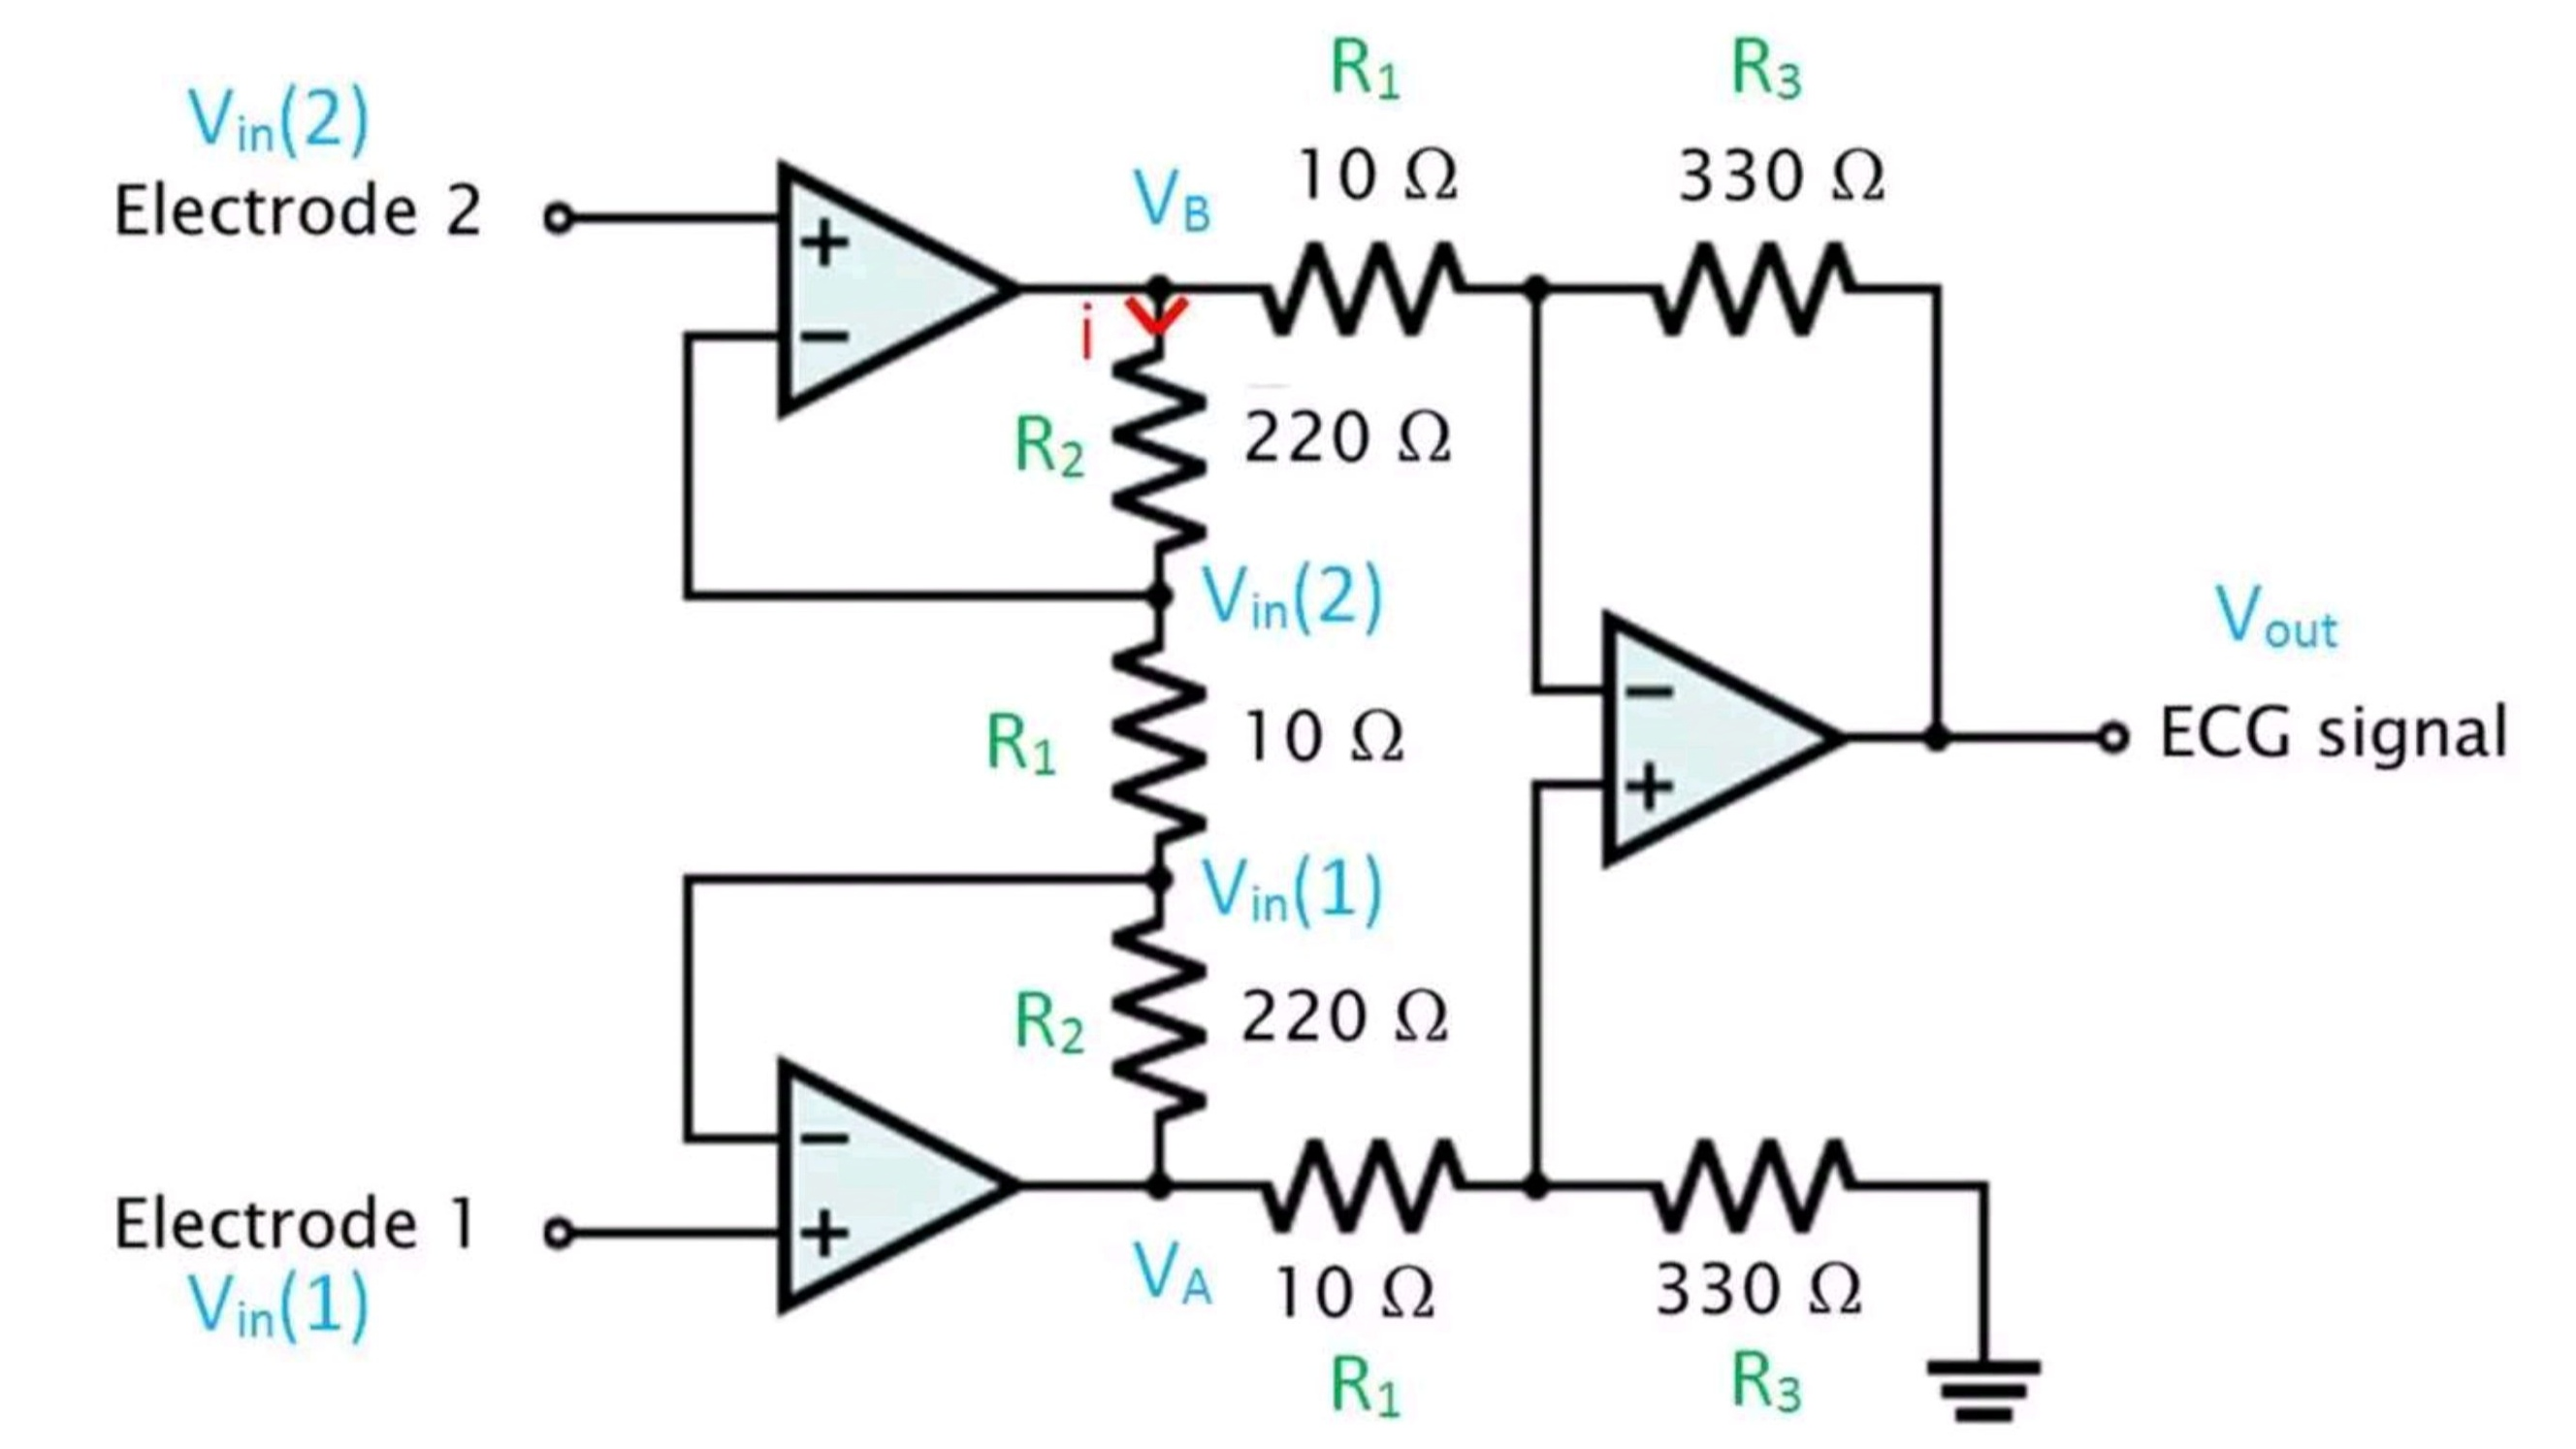
\includegraphics[width=0.7\textwidth]{images/bio_Ins.jpg}
        \caption{BioInstrumentation Amplifier topology}
        \label{fig:bioIns_block}
    \end{figure}
    \item Internal high-pass (0.5 Hz) and low-pass (~40 Hz) filters for motion and line noise rejection.
\end{itemize}

\section{AMPLIFIER}
We use the AD8232\cite{AD8232} bioinstrumentation amplifier, a reliable choice for portable ECG devices. This amplifier is designed to capture the heart’s weak electrical signals and amplify them for accurate processing. It offers high precision, low power consumption, and effective signal enhancement, making it suitable for mobile applications where battery efficiency and signal clarity are crucial.
\begin{figure}[H]
    \centering
    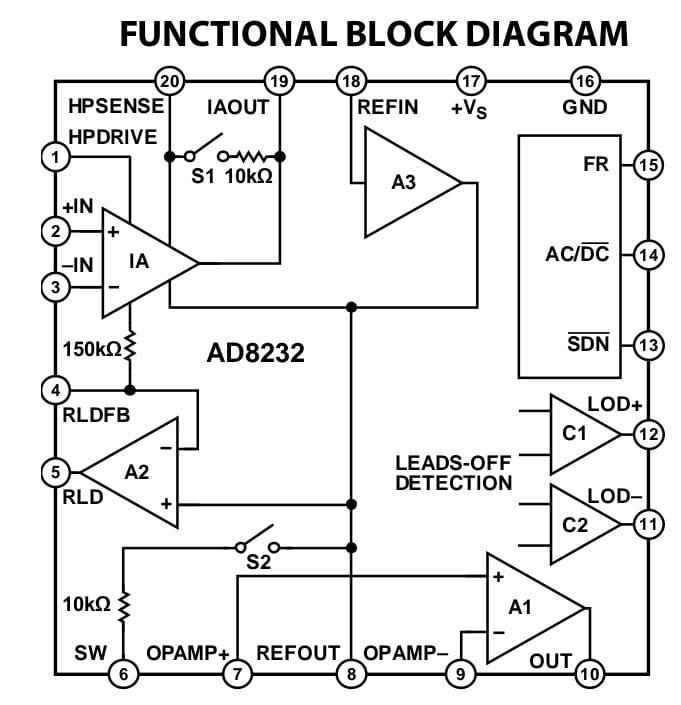
\includegraphics[width=0.7\textwidth]{images/ad8232_block.jpg}
    \caption{AD8232 block diagram\cite{AD8232}}
    \label{fig:AD8232_block}
\end{figure}

\textbf{Additional Filtering:}
\begin{itemize}
    \item \textbf{RC low-pass filter:} After AD8232 output, an RC filter (typically 1kΩ + 10$\mu$F) suppresses 50/60Hz hum.
    \item \textbf{Decoupling capacitors:} Used near the supply rails for stability.
\end{itemize}

\begin{figure}[H]
    \centering
    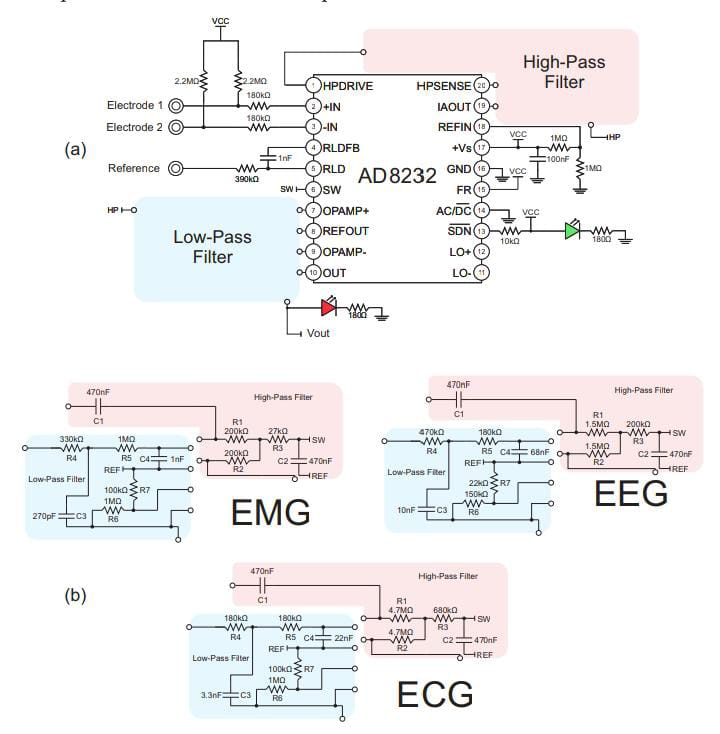
\includegraphics[width=0.6\textwidth]{images/ad8232_circuit.jpg}
    \caption{AD8232 circuit diagram\cite{AD8232}}
    \label{fig:AD8232_circuit}
\end{figure}

\section{Power Supply}
\begin{itemize}
    \item \textbf{Battery:} 1200mAh Li-ion, securely fixed inside the enclosure.
    \item \textbf{Charging Circuit:} TP4056-based charger IC with overcurrent protection.
    \item \textbf{Voltage Regulation:} External LDO of RT9080 - 3.3v used; draws ~120mA peak with WiFi.
\end{itemize}

\section{Enclosure and Controls}
\begin{itemize}
    \item \textbf{Heart Symbol LED:} Located at top-center, pulses with heart rhythm and indicates power.
    \item \textbf{Charge-Off-On switch:} Controls power flow.
    \item \textbf{Red LED:} Glows during charging.
    \item \textbf{Blue LED:} Indicates full charge.
\end{itemize}






\chapter{Signal Acquisition and Filtering}

\section{Signal Characteristics}
Typical ECG voltages are 0.5–3 mV, requiring careful amplification. The AD8232 amplifies these small signals to ~1V peak-to-peak for easy sampling by the 10-bit ADC of the ESP8266.

\section{ADC Considerations}
\begin{itemize}
    \item ESP8266 ADC reads 0–1V with 10-bit resolution.
    \item An external voltage divider biases the analog input to ~0.5V baseline (AC-coupled).
    \item The effective resolution is $\frac{1V}{1024} \approx 0.976mV$ per ADC step.
\end{itemize}

\section{Filtering Pipeline}
\textbf{Hardware Filtering:}
\begin{itemize}
    \item High-pass (0.5 Hz) to eliminate baseline wander (from respiration).
    \item Low-pass (~40 Hz) to remove muscle noise.
\end{itemize}

\textbf{Frontend JS Filtering:}
\begin{itemize}
    \item Rolling average (N = 5 to 10 samples).
    % \item Optional digital IIR high-pass to stabilize drift.
\end{itemize}

\section{Noise Sources Addressed}
\begin{itemize}
    \item \textbf{Power Line Noise:} Minimized by RC filter + good PCB routing.
    \item \textbf{Motion Artifact:} Reduced via chest electrodes and tight contact.
    % \item \textbf{EMI:} Shielded wiring and star grounding reduce interference.
\end{itemize}






\chapter{Software Architecture}

\section{ESP8266 Firmware Design}
Firmware is written using the Arduino core for ESP8266. Major modules include:
\begin{itemize}
    \item \textbf{WiFi Access Point:} Default SSID “Micro\_ECG\_RANMPGroupF”, no password.
    \item \textbf{Captive Portal:} Uses DNS hijack and local HTTP server.
    \item \textbf{WebSocket Server:} For real-time ADC streaming.
    \item \textbf{ADC Sampling:} Samples analog ECG at ~250Hz using a timer interrupt.
    \item \textbf{Frame Batching:} Sends 70-80 samples per WebSocket frame for efficiency.
\end{itemize}

\begin{figure}[H]
\centering
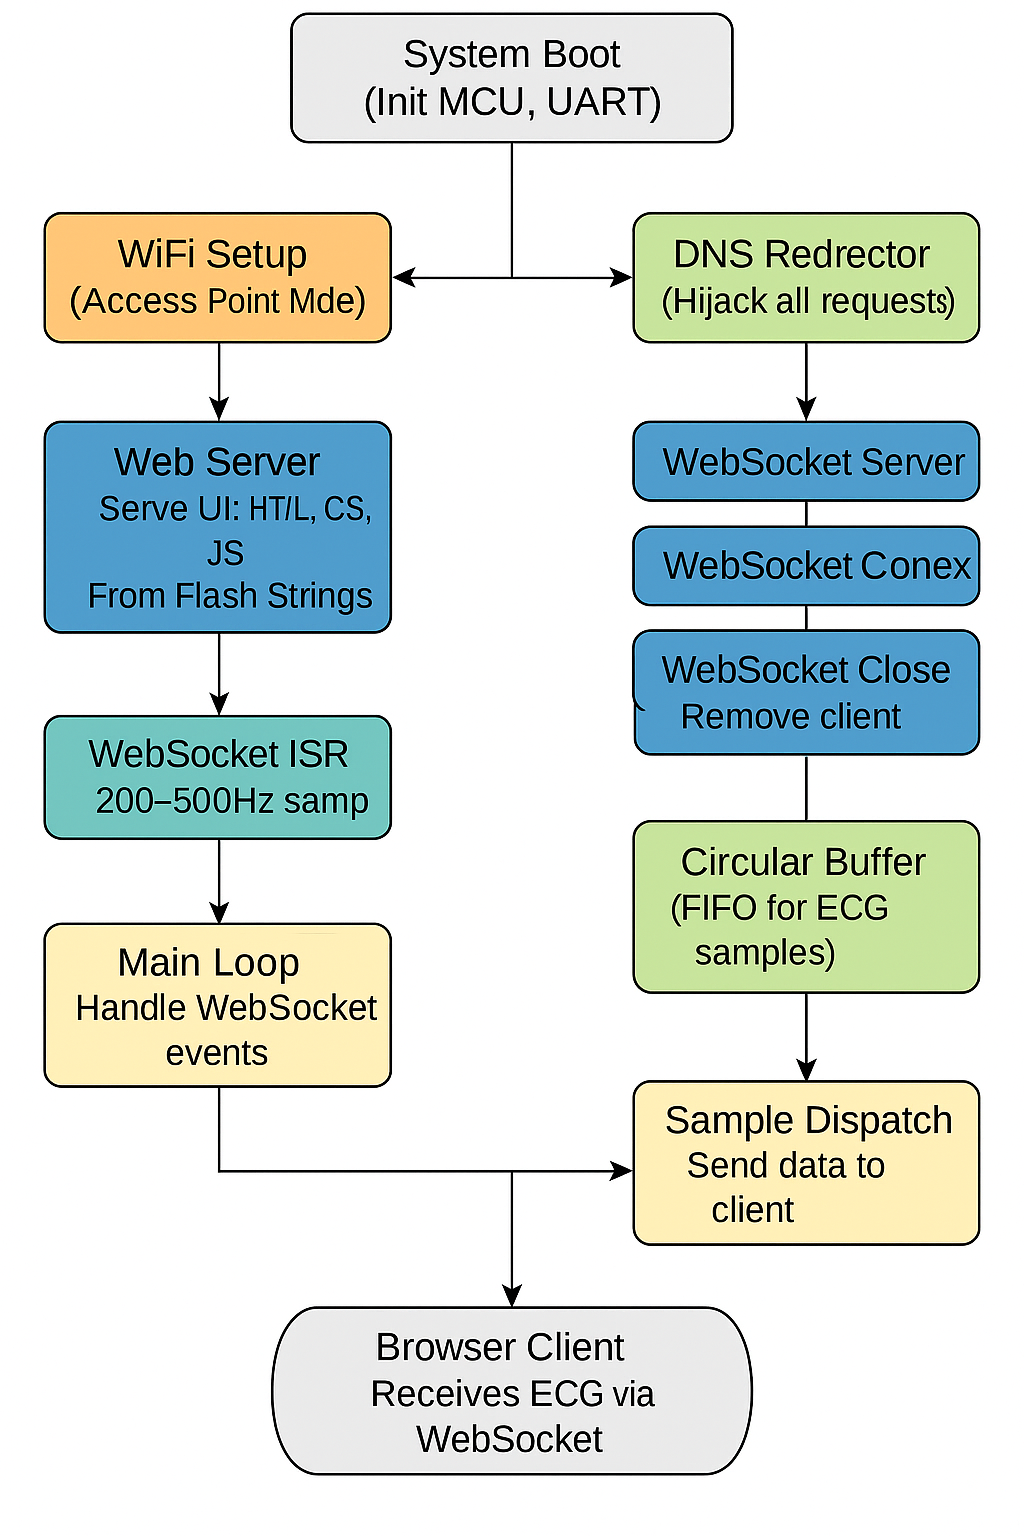
\includegraphics[width=0.6\textwidth]{images/firmware-diagram(8266).png}
\caption{ESP8266 Firmware Architecture}
\label{fig:firm8266_diagram}
\end{figure}


\section{Sampling Optimization}
\begin{itemize}
    \item ADC read in ISR (Interrupt Service Routine) using \texttt{timer1}.
    \item Samples placed into ring buffer.
    \item Main loop dispatches WebSocket events and serves UI files.
\end{itemize}

\section{OTA and Updates}
Firmware updates are performed via USB using Espressif Flash Download Tools [see official documentation from https://www.espressif.com/en ].






\chapter{Frontend Web User Interface}

\section{Architecture Overview}
The frontend is written in plain HTML5, CSS, and JavaScript, hosted locally from ESP8266 flash. No backend or internet is required. The user connects to the device via WiFi, and the interface is served directly.

\begin{figure}[H]
\centering
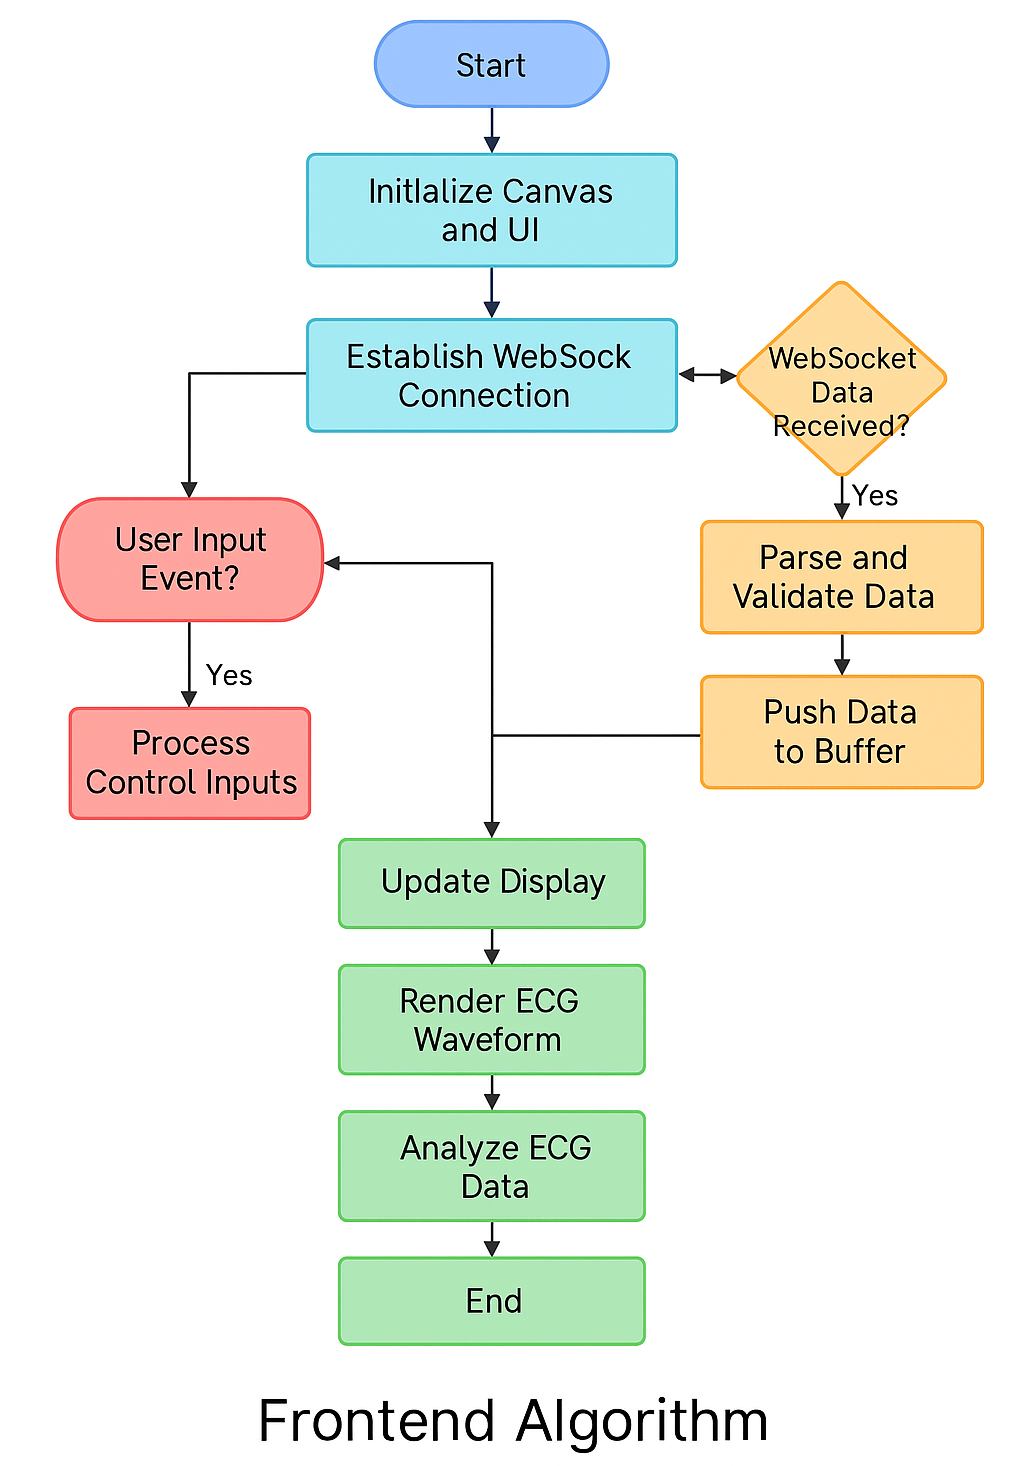
\includegraphics[width=0.6\textwidth]{images/firmware-diagram(frontend).png}
\caption{Frontend Firmware Architecture}
\label{fig:firm_frontend_diagram}
\end{figure}

\section{Canvas Rendering Engine}
The ECG signal is plotted on an HTML5 `<canvas>` element. Core design:
\begin{itemize}
    \item \textbf{Canvas Width:} Responsive; typically 300–1200px or more depending on device screen.
    % \item \textbf{Y-Scale Calculation:} Autoscaled to keep peak-to-peak signal visible.
    \item \textbf{X-Axis Mapping:} Buffer size determines how many samples fit on screen.
    % \item \textbf{Grid Lines:} Vertical (time divisions), Horizontal (amplitude markers).
\end{itemize}

\section{Signal Buffer Handling}
\begin{itemize}
    \item Uses a JavaScript array (`data\_buffer[]`) to hold recent ADC values.
    \item Buffer size is set to match screen width (e.g., 1000 samples = 5s window at 200Hz).
    \item Incoming WebSocket samples are pushed, old values popped.
    \item Dynamic range detection adjusts gain (volts/div) and vertical centering.
\end{itemize}

\section{Filtering and Scaling}
\begin{itemize}
    \item Basic smoothing via moving average (optional toggle).
    \item JavaScript-based digital high-pass for baseline correction.
    % \item Y-axis scale auto-adjusts to match incoming waveform amplitude.
\end{itemize}

\section{Event Handling}
\begin{itemize}
    \item \textbf{Resize Event:} Rescales canvas and resets buffer.
    % \item \textbf{Touch Support:} Can add tap-to-freeze or mark timestamps.
    \item \textbf{Error Events:} Notifies disconnection, reconnection, or invalid data.
\end{itemize}

\section{AI Integration}
\begin{itemize}
    \item The frontend can connect to a third-party ECG AI API.
    \item Sample batch is sent as JSON POST.
    \item Resulting classification (e.g., normal/AFib) is shown below the canvas in AI tab.
    \item Used for advanced diagnostics, requires internet access.
\end{itemize}






\chapter{User Operation Guide}

\section{Getting Started}
\subsection{Power On}
Slide \textbf{POWER} switch to ON. The heart LED should start blinking.
(If it doesn't blink, ensure the device is charged.)
\subsection{Connect to Wi-Fi}
On your mobile or computer, connect to the device’s Wi-Fi hotspot.
(Note: Only supports 2.4GHz networks.)
\subsection{Open the User Interface}
Once connected to the ECG device's Wi-Fi, a screen should automatically pop up with the web interface. \\
If it doesn’t open by itself, just open any browser (Chrome recommended) and go to: \\
http://172.217.28.1 \\
Chrome tested on mobile, desktop, and laptop — works on cross-platform.
\subsection{ECG Display}
The graph canvas may initially show random noise if electrodes are open.

\subsection{Electrodes}
\begin{itemize}[leftmargin=*]
  \item \textbf{Finger:} Touch LA \& RA on top of the device. OR,
  \item \textbf{Chest:} Connect external electrode (Front-Left side)
\end{itemize}

\subsection{Take Reading}
Once the waveform is stable , no noise on the screen, hold still and observe the heart rate.

\section{Parameters}
\begin{figure}[H]
    \centering
    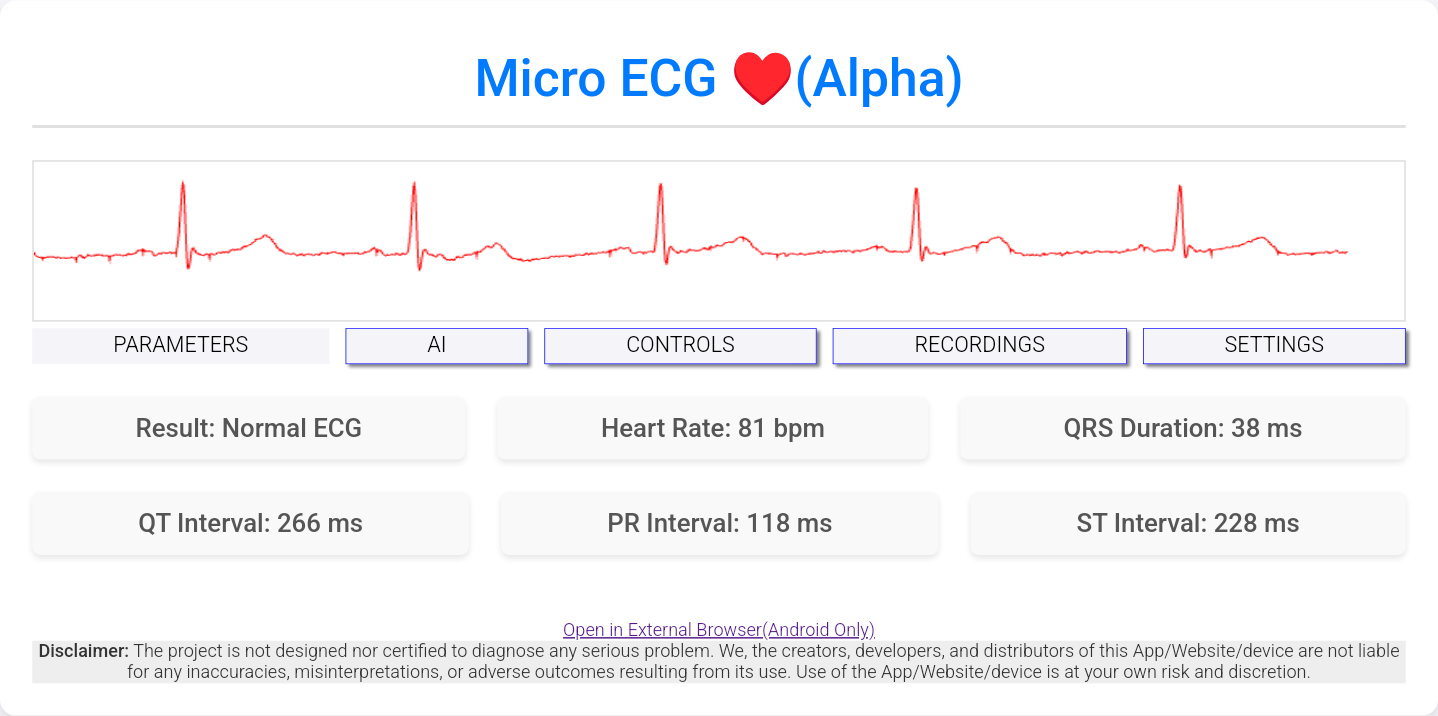
\includegraphics[width=0.7\textwidth]{images/ss/view-param.png}
    \caption{User interface Parameters view}
    \label{fig:ss_param_view}
\end{figure}
\begin{itemize}[leftmargin=*]
    \item \textbf{Heart Rate (BPM):} -  Beats per minute calculated in real-time.
    \item \textbf{QRS Duration:} -  Time interval of the QRS complex, indicating ventricular depolarization.
    \item \textbf{QT Interval:} -  Total time for ventricular depolarization and repolarization.
    \item \textbf{PR Interval:} -  Time from the start of the P wave to the start of the QRS complex.
    \item \textbf{ST Interval:} -  Segment between the end of the S wave and the beginning of the T wave.
\end{itemize}

\section{AI Assistant}
\begin{figure}[H]
    \centering
    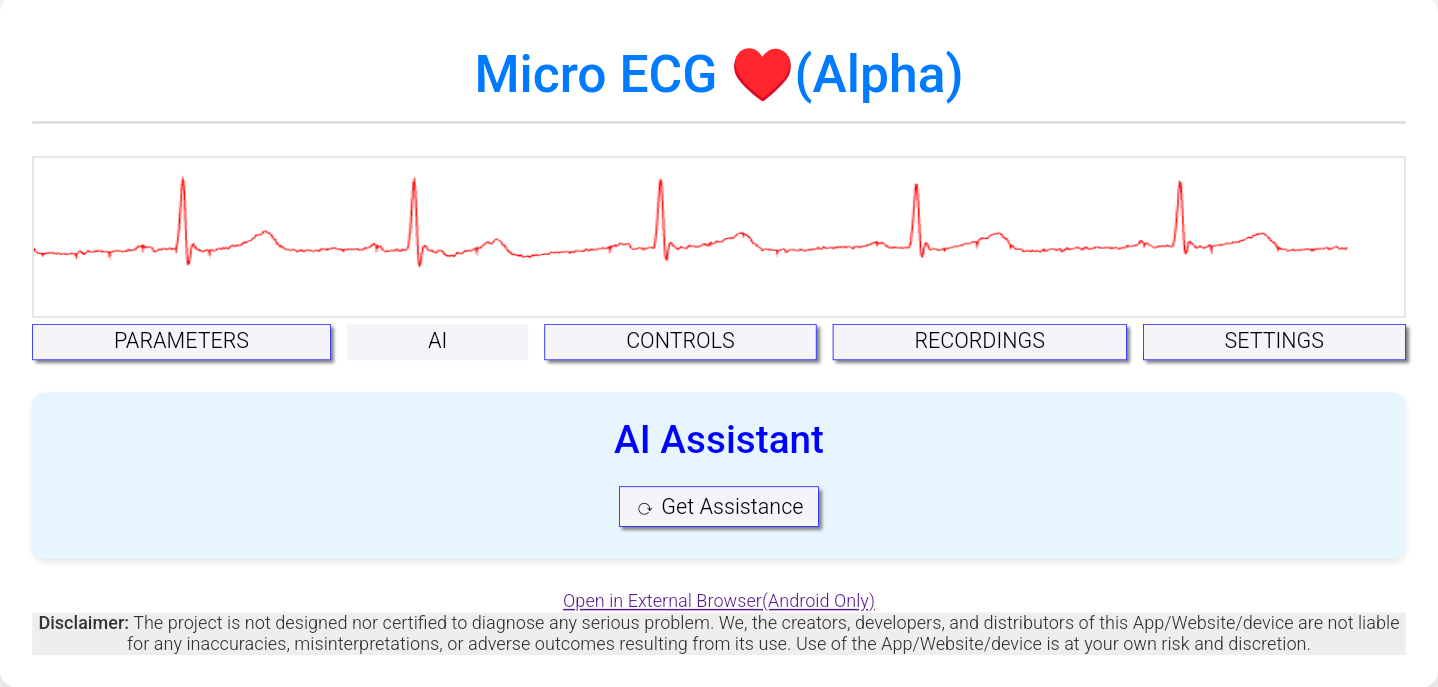
\includegraphics[width=0.7\textwidth]{images/ss/view-ai.png}
    \caption{User interface AI view}
    \label{fig:ss_ai_view}
\end{figure}
\begin{itemize}[leftmargin=*]
    \item \textbf{Function:} -  ECG data send to a third-party AI for anomaly detection.
    \item \textbf{How to Use:} -  Click on the "Get Assistance" button to initiate the AI analysis.
\end{itemize}

\section{Controls}
\begin{figure}[H]
    \centering
    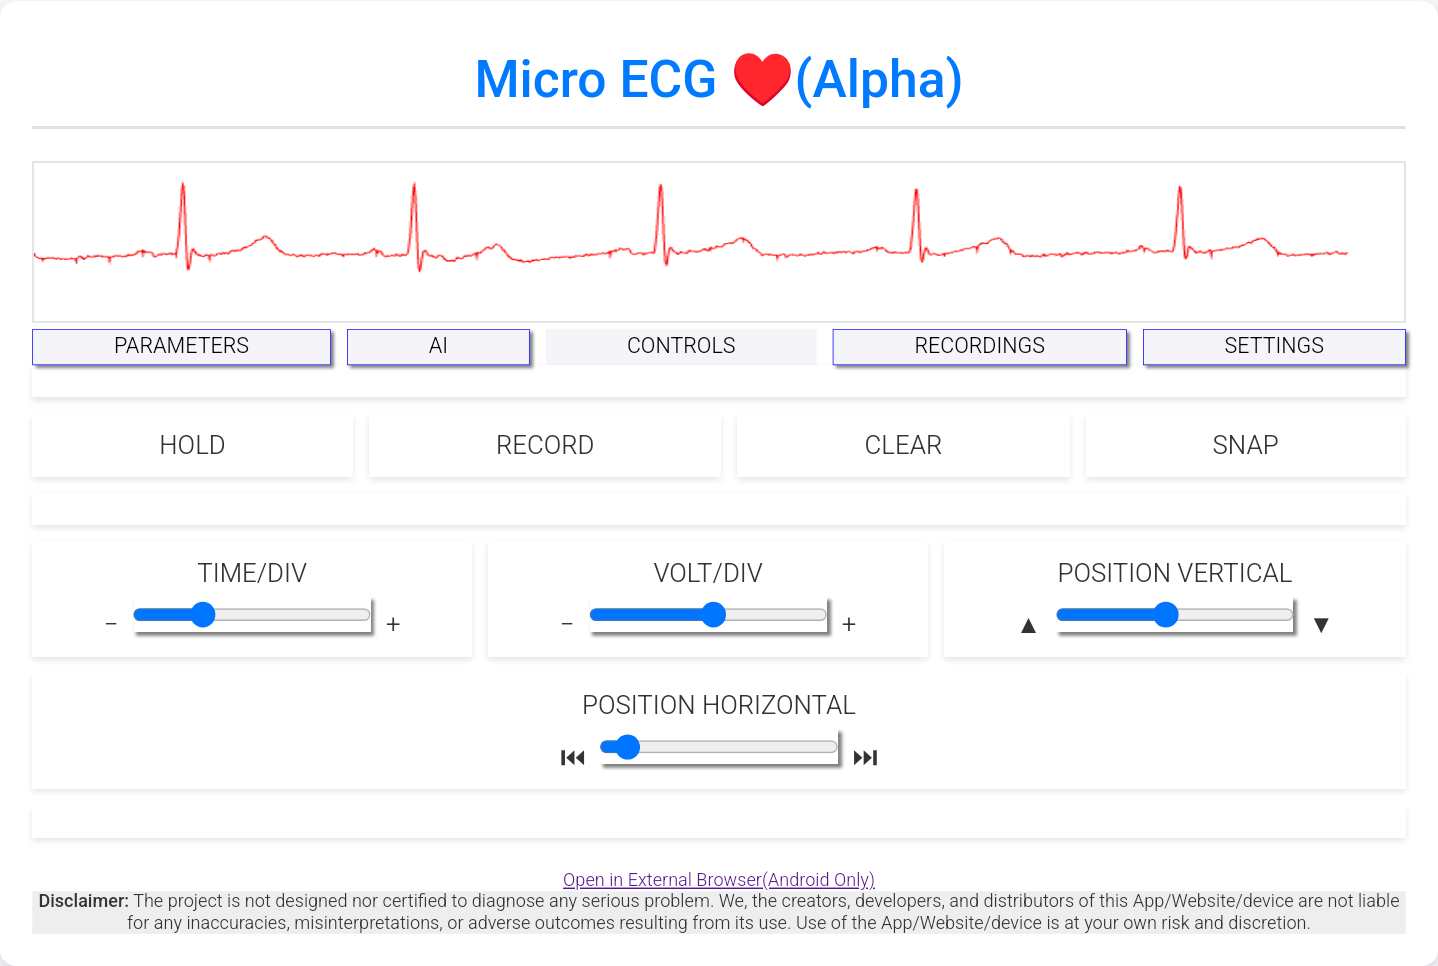
\includegraphics[width=0.7\textwidth]{images/ss/view-controls.png}
    \caption{User interface Controls view}
    \label{fig:ss_controls_view}
\end{figure}
\begin{itemize}[leftmargin=*]
    \item \textbf{HOLD:} -  Pauses the real-time ECG display.​
    \item \textbf{RECORD:} -  Starts recording the ECG data.​
    \item \textbf{CLEAR:} -  Clears the current ECG graph from the display.​
    \item \textbf{SNAP:} -  Captures a snapshot of the current ECG graph.​
    \item \textbf{TIME/DIV (-/+):} -  Adjusts the time scale of the ECG graph.​
    \item \textbf{VOLT/DIV (-/+):} -  Adjusts the voltage scale of the ECG graph.
    \item \textbf{POSITION VERTICAL (\ding{115}/\ding{116}):} -  Moves the ECG graph up or down.​
    \item \textbf{POSITION HORIZONTAL (\prevtrack/\nexttrack):} -  Moves the ECG graph left or right.​
\end{itemize}

\section{Recordings}
\begin{figure}[H]
    \centering
    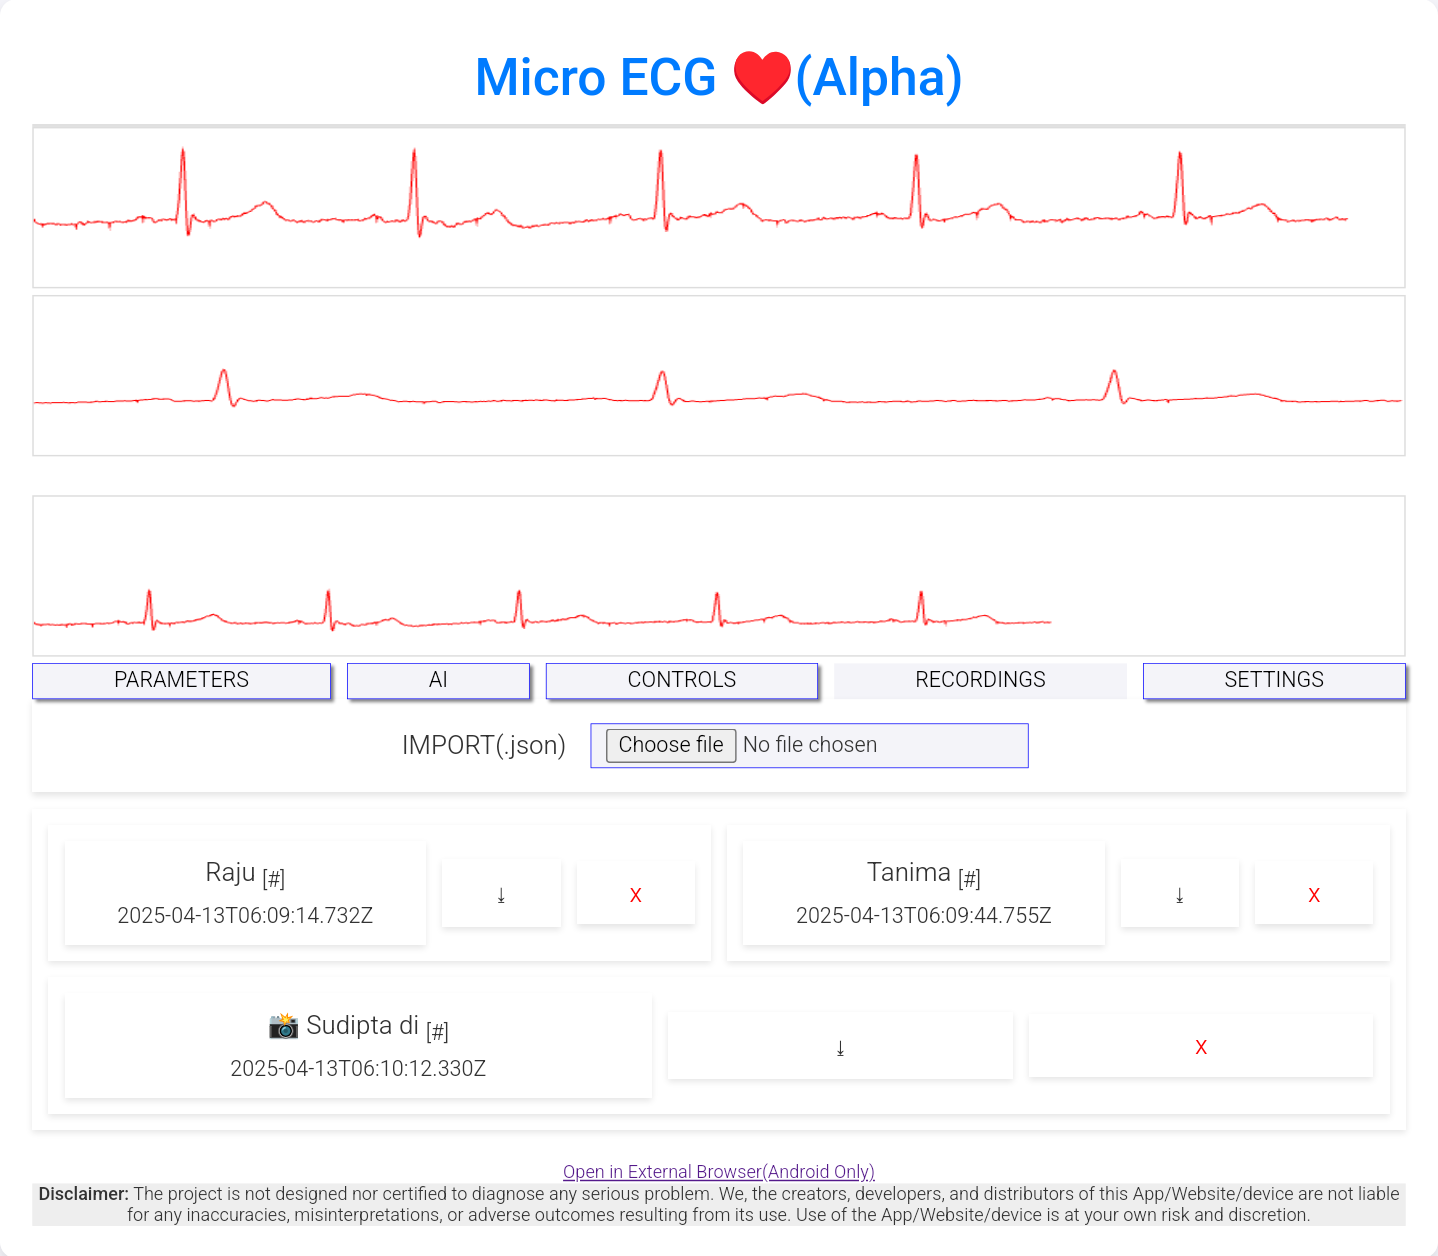
\includegraphics[width=0.7\textwidth]{images/ss/view-record.png}
    \caption{User interface Recordings view}
    \label{fig:ss_record_view}
\end{figure}
\begin{itemize}[leftmargin=*]
    \item \textbf{IMPORT (.json):} -  Allows importing of ECG data in JSON format.
    
    \item \textbf{Accessing Recordings:} -  Recorded ECG sessions are listed with timestamps in the RECORDINGS section..​
    \item \textbf{Downloading Recordings:} -  Click on the download (\downleftarrow) icon next to a recording to download the data..​
    \item \textbf{Deleting Recordings:} -  Click on the ($\times$) icon next to a recording to delete it.
\end{itemize}

\section{Settings (Not available - Planned)}
% \begin{itemize}[leftmargin=*]
%   \item WiFi SSID change
%   \item Adjust SPS
%   \item Factory Reset
%   \item Firmware update access
% \end{itemize}

\section{Troubleshooting}
\begin{itemize}
    \item \textbf{No Heart LED Blinking:} \\
    Ensure the device is charged. Slide the power switch OFF and ON again.

    \item \textbf{Cannot Connect to Wi-Fi:} \\
    Confirm your device supports 2.4GHz Wi-Fi. Restart the ECG device and try again.

    \item \textbf{Web Interface Doesn’t Open Automatically:} \\
    Check sign-in notification | open a browser manually (Chrome recommended) and enter\\ \texttt{http://172.217.28.1}.

    \item \textbf{Weak signal:} \\
    Possible Cause: Dry skin, poor contact | Moisten fingers slightly or use external electrode.

    \item \textbf{Data delay in UI:} \\
    Improve WiFi signal, Move closer to the device.

    \item \textbf{ECG Graph Shows Noise:} \\
    Ensure stable positioning, avoid movement. \\
    Make sure the electrodes are placed correctly. Wait a few seconds for the signal to stabilize. \\
    For finger electrodes, gently rub and clean the metal surface before use to improve contact. \\
    \textbf{Do not} try to rub or clean the disposable adhesive external electrodes, as this may damage them.
\end{itemize}

\section{Safety \& Maintenance}
\begin{itemize}[leftmargin=*]
  \item Keep electrodes clean and dry for optimal signal quality.
  \item Use BIS certified charger to charge via Micro-USB.
  \item Do not submerge in water or expose to excessive moisture.
  \item Don't drop or shake.
  \item Update firmware from authorised source only.
  \item Avoid applying excessive force on the device or electrodes.
\end{itemize}












\chapter{Implementation and Results}

\section{Prototype Construction}
The entire circuit—including the AD8232, ESP8266 module, charging system, and control switch—was soldered with Enameled Copper Wire and enclosed in a non-conductive plastic case. Design priorities:
\begin{itemize}
    \item Minimal footprint (pocket-sized, ~13cm x 4cm x 4cm).
    \item Direct finger placement for LA/RA.
    \item Access to external chest port.
    \item Long battery life with charging.
\end{itemize}

\begin{figure}[h]
    \centering
    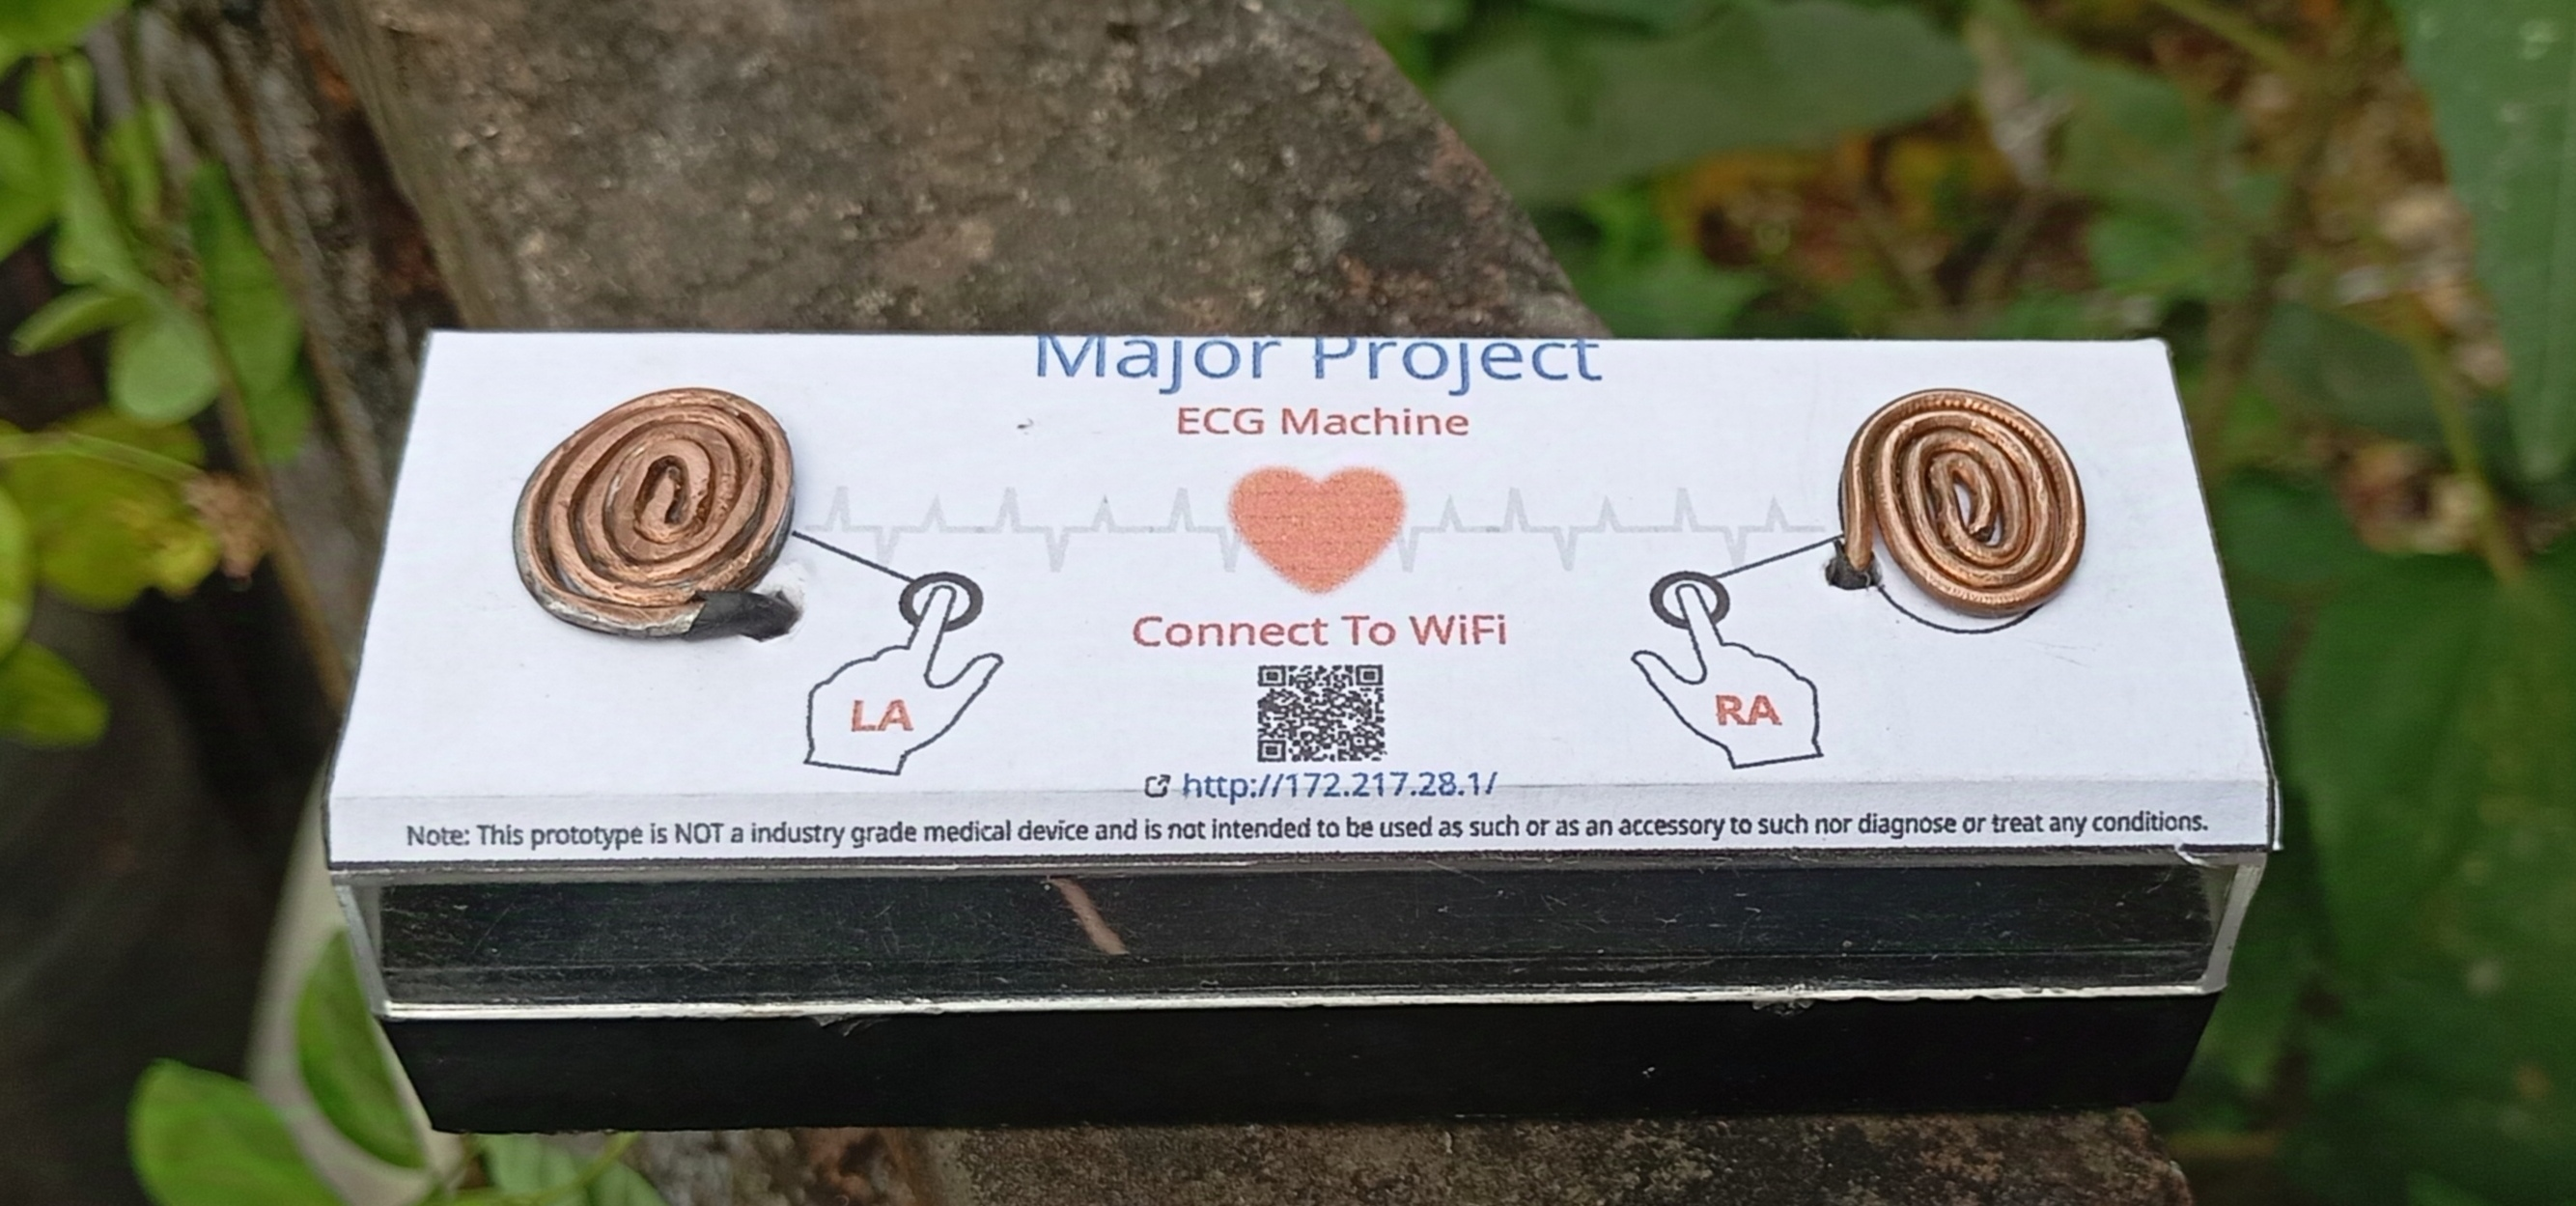
\includegraphics[width=0.75\textwidth]{images/proto.jpg}
    \caption{Final device prototype}
\end{figure}

% \section{PCB Layout Overview}
% The PCB includes separate analog and digital ground planes to minimize interference. Analog paths are shielded and routed first. The ESP8266 is mounted centrally to reduce trace length for ADC signal.

\section{Signal Stability and Noise Test}
Tests were conducted using both finger and chest electrodes. Observations:
\begin{itemize}
    \item With proper finger placement, the R-peaks are clearly visible.
    \item Chest lead usage significantly reduced baseline drift.
    \item Minor noise was handled via JavaScript-based smoothing.
\end{itemize}

\section{Web Interface Performance}
\begin{itemize}
    \item Tested on Android, iOS, Windows, and Linux.
    \item Average frame rate: ~15 fps(matches base device screen fps) with 200Hz data.
    \item Latency between ADC read and graph render: <500ms.
    \item No buffering issues observed during continuous 30-minute sessions.
\end{itemize}

\begin{figure}[h]
    \centering
    \begin{subfigure}[b]{0.45\textwidth}
        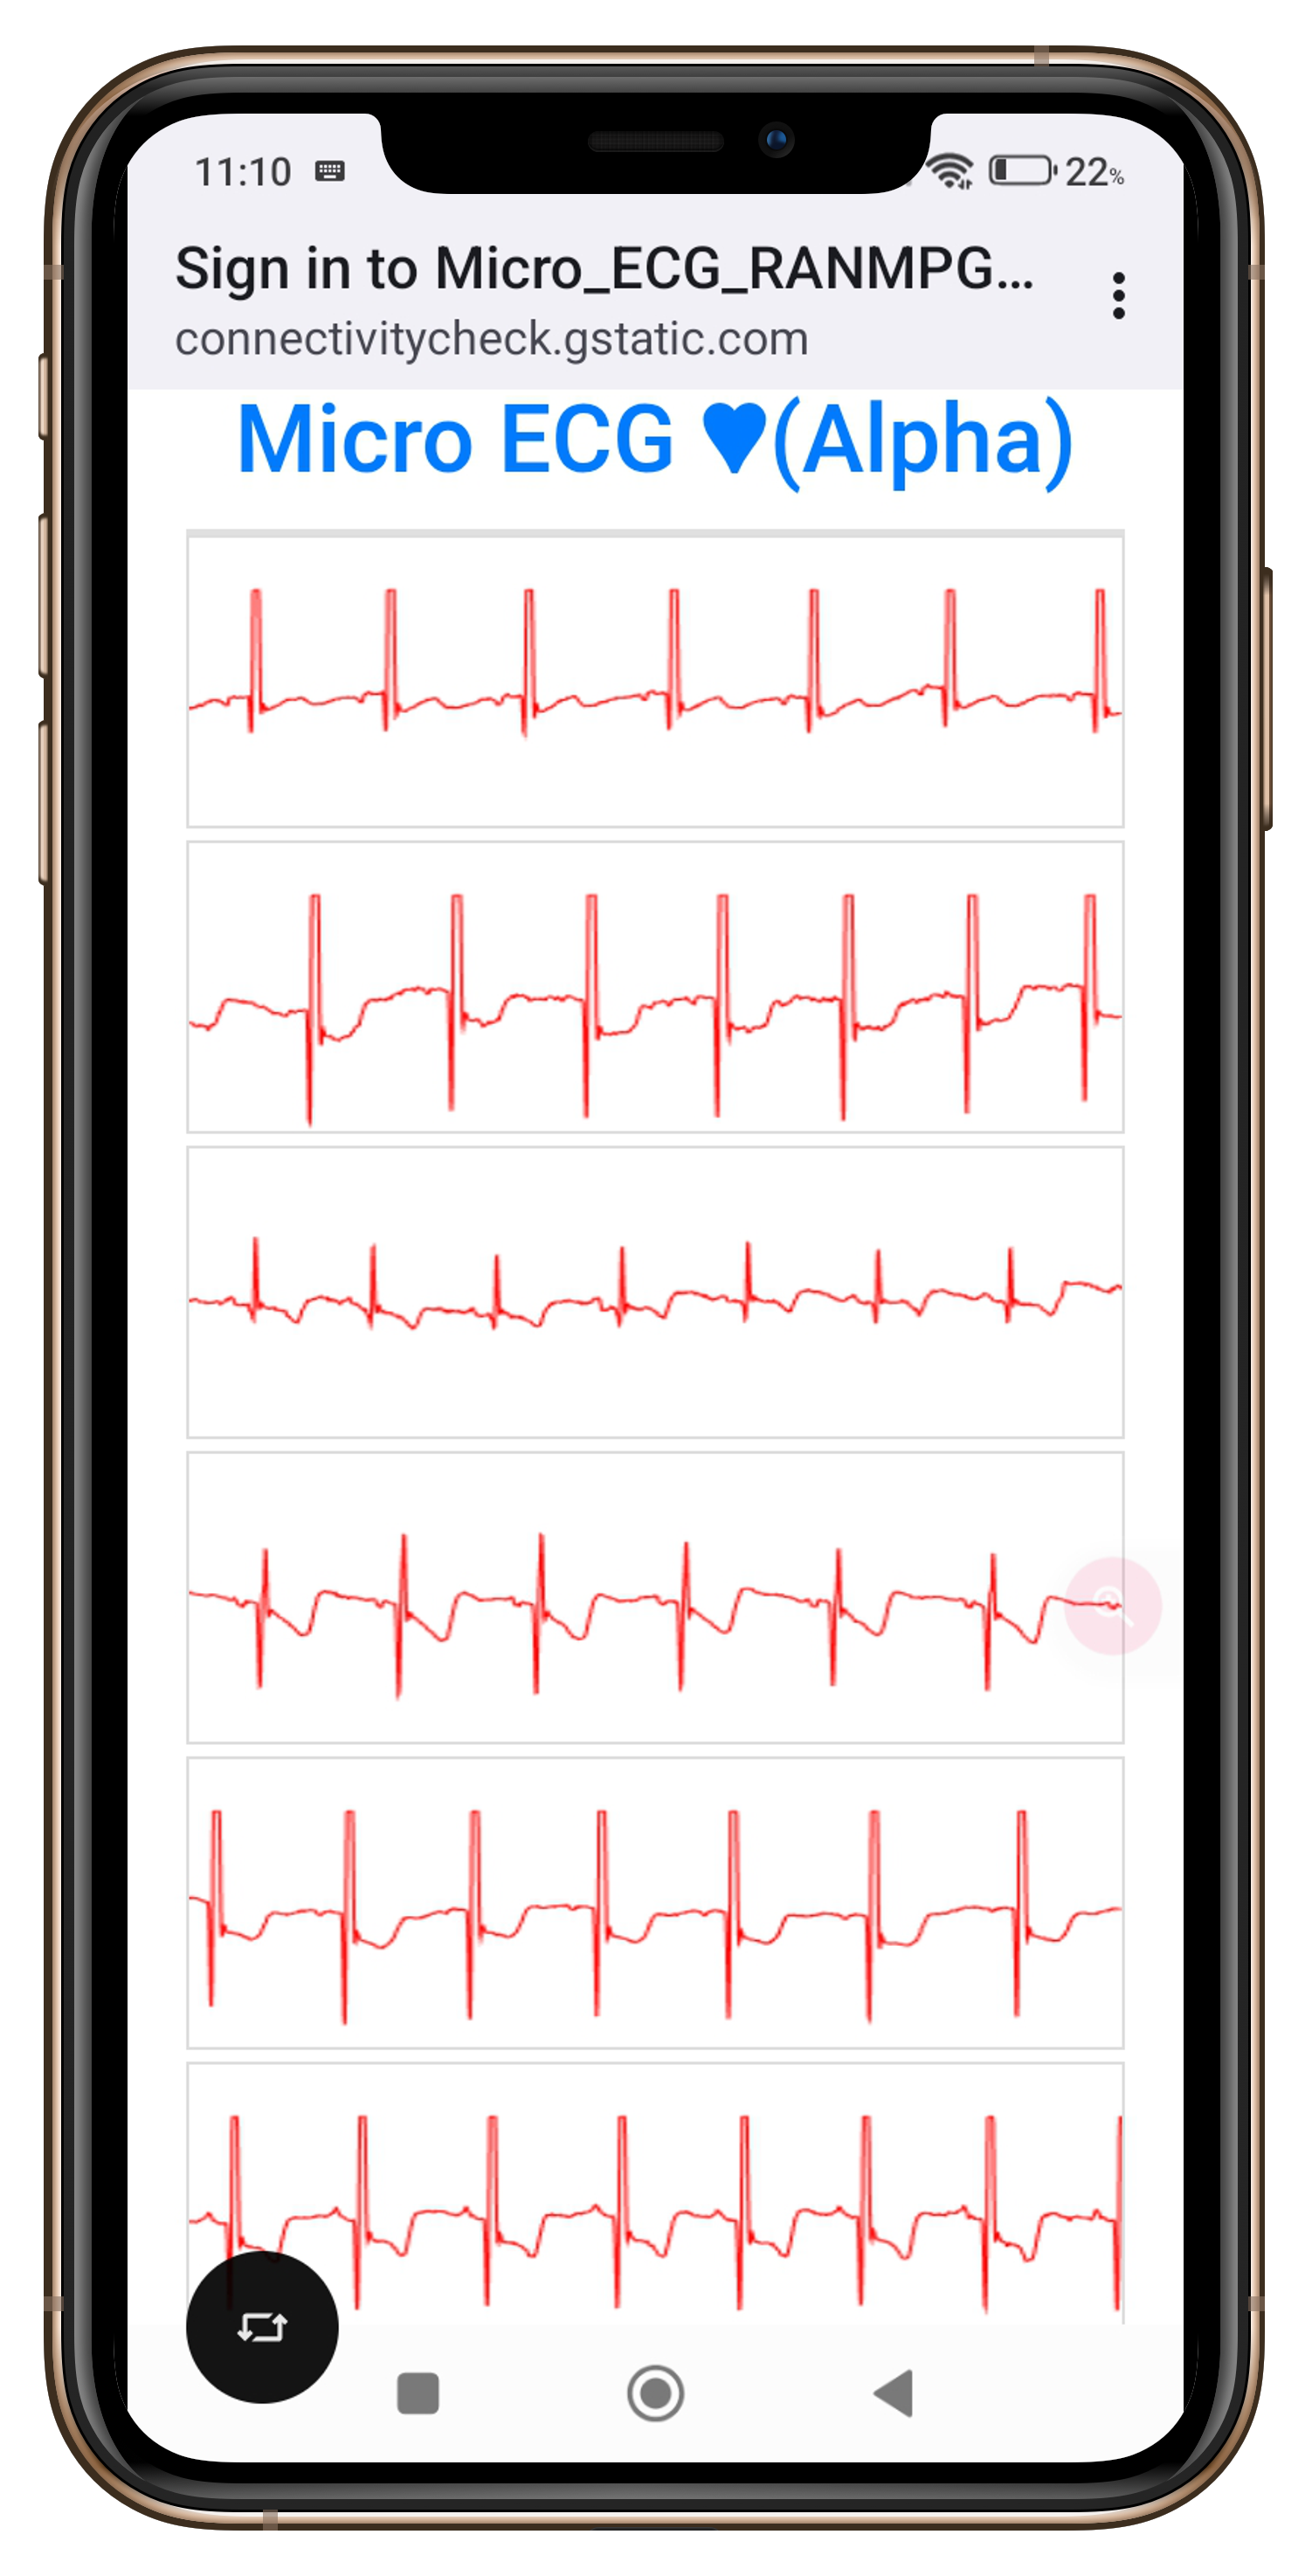
\includegraphics[width=\textwidth]{images/result-portrait.png}
        \caption{ECG signal rendering on browser from 6 different leads}
    \end{subfigure}
    \hfill
    \begin{subfigure}[b]{0.45\textwidth}
        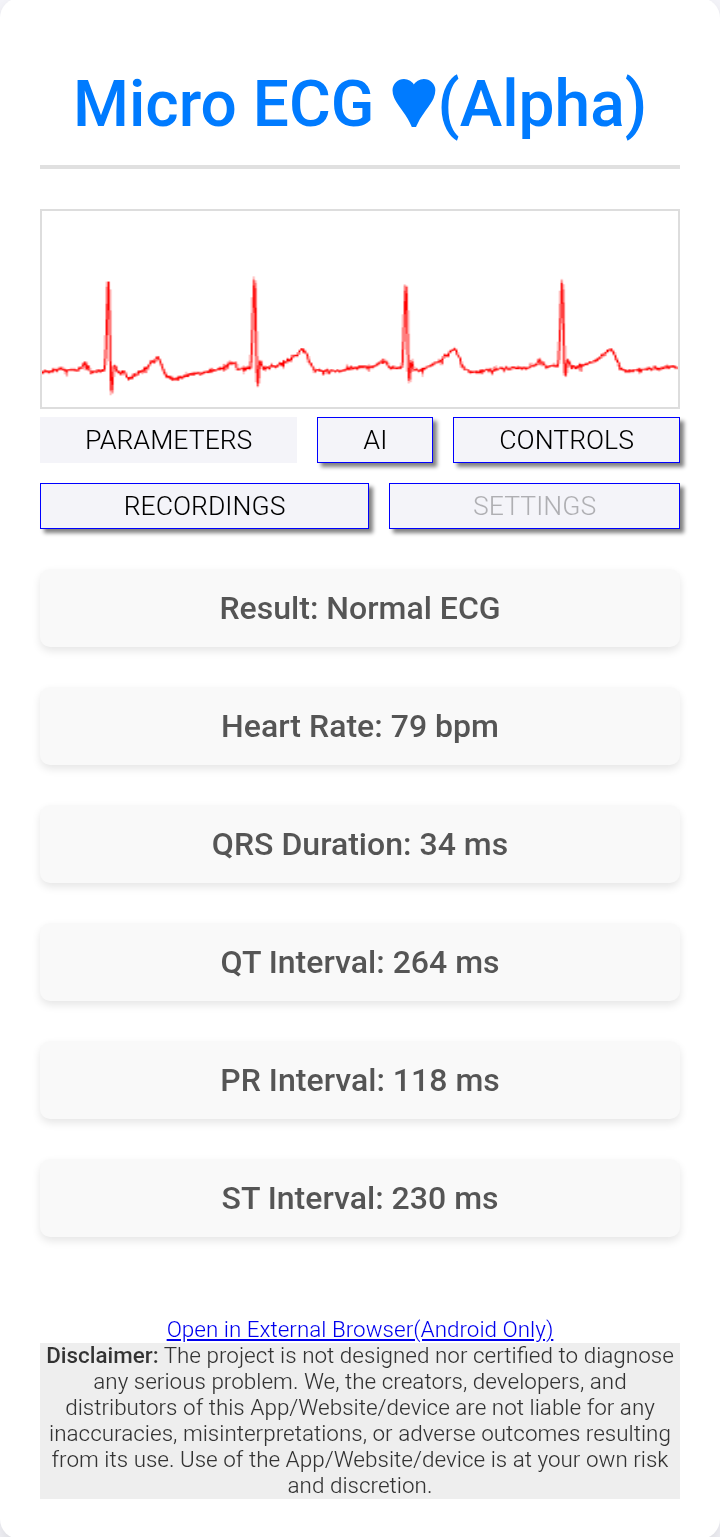
\includegraphics[width=\textwidth]{images/result-params.png}
        \caption{ECG signal parameters automatic algorithmic analysis}
    \end{subfigure}
    \caption{ECG signal and parameters - RESULT}
\end{figure}
\begin{figure}
    \centering
    \begin{subfigure}[b]{0.45\textwidth}
        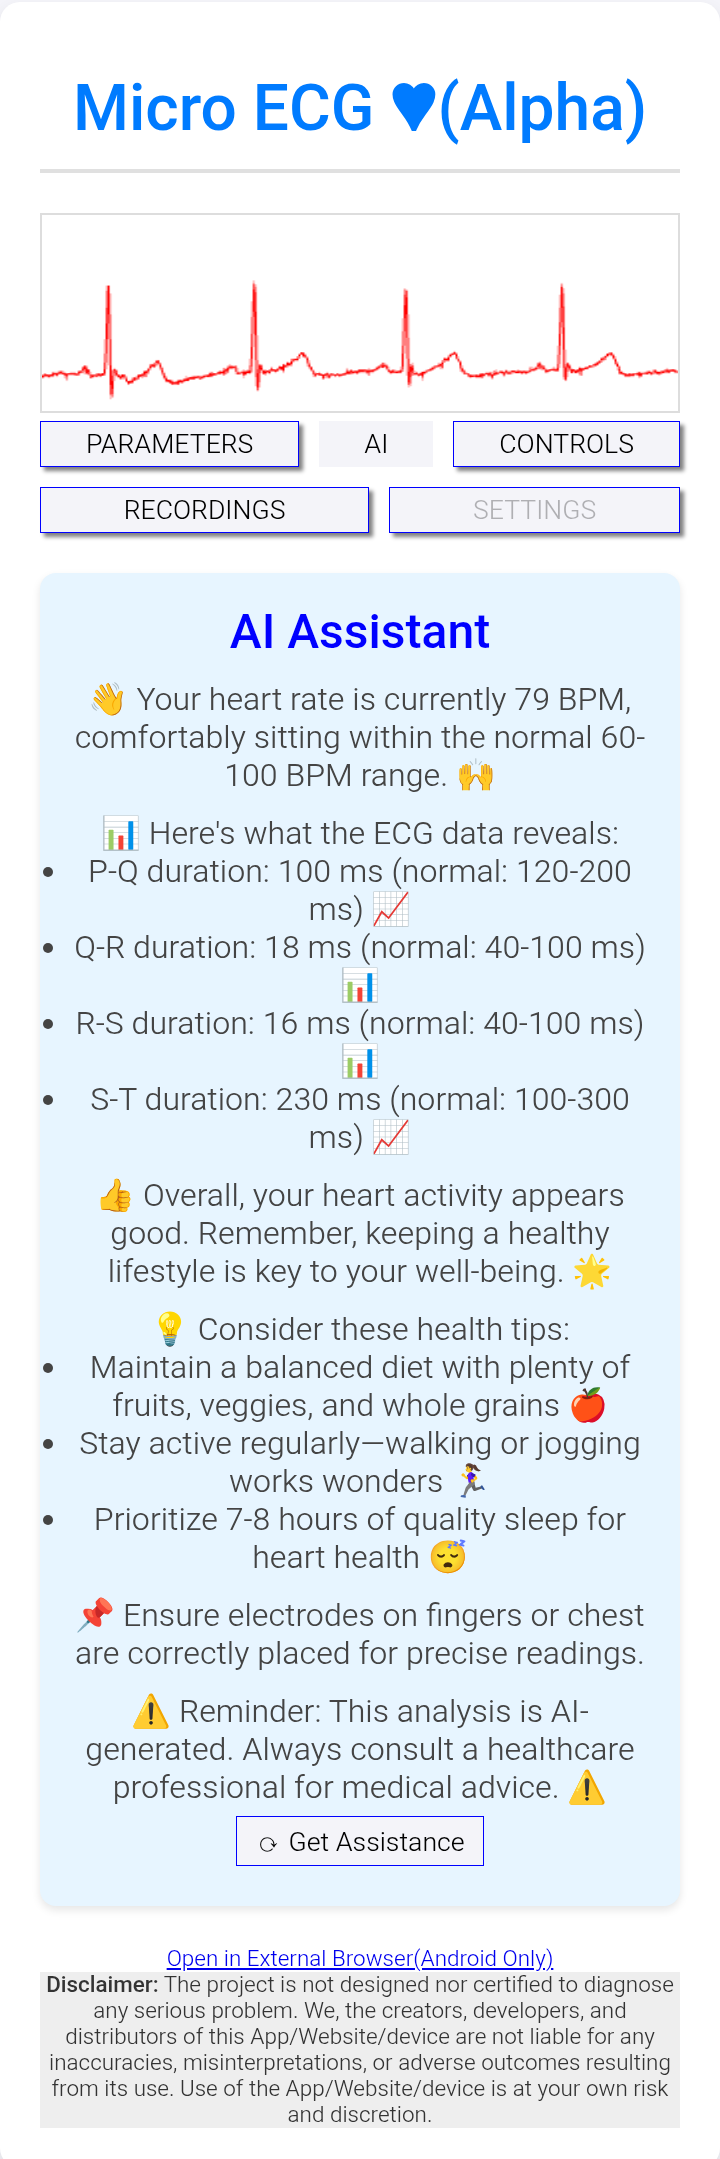
\includegraphics[width=\textwidth]{images/result-AI.png}
        \caption{ECG signal AI Analysis from third-party AI agent API endpoint}
    \end{subfigure}
    \hfill
    \begin{subfigure}[b]{0.45\textwidth}
        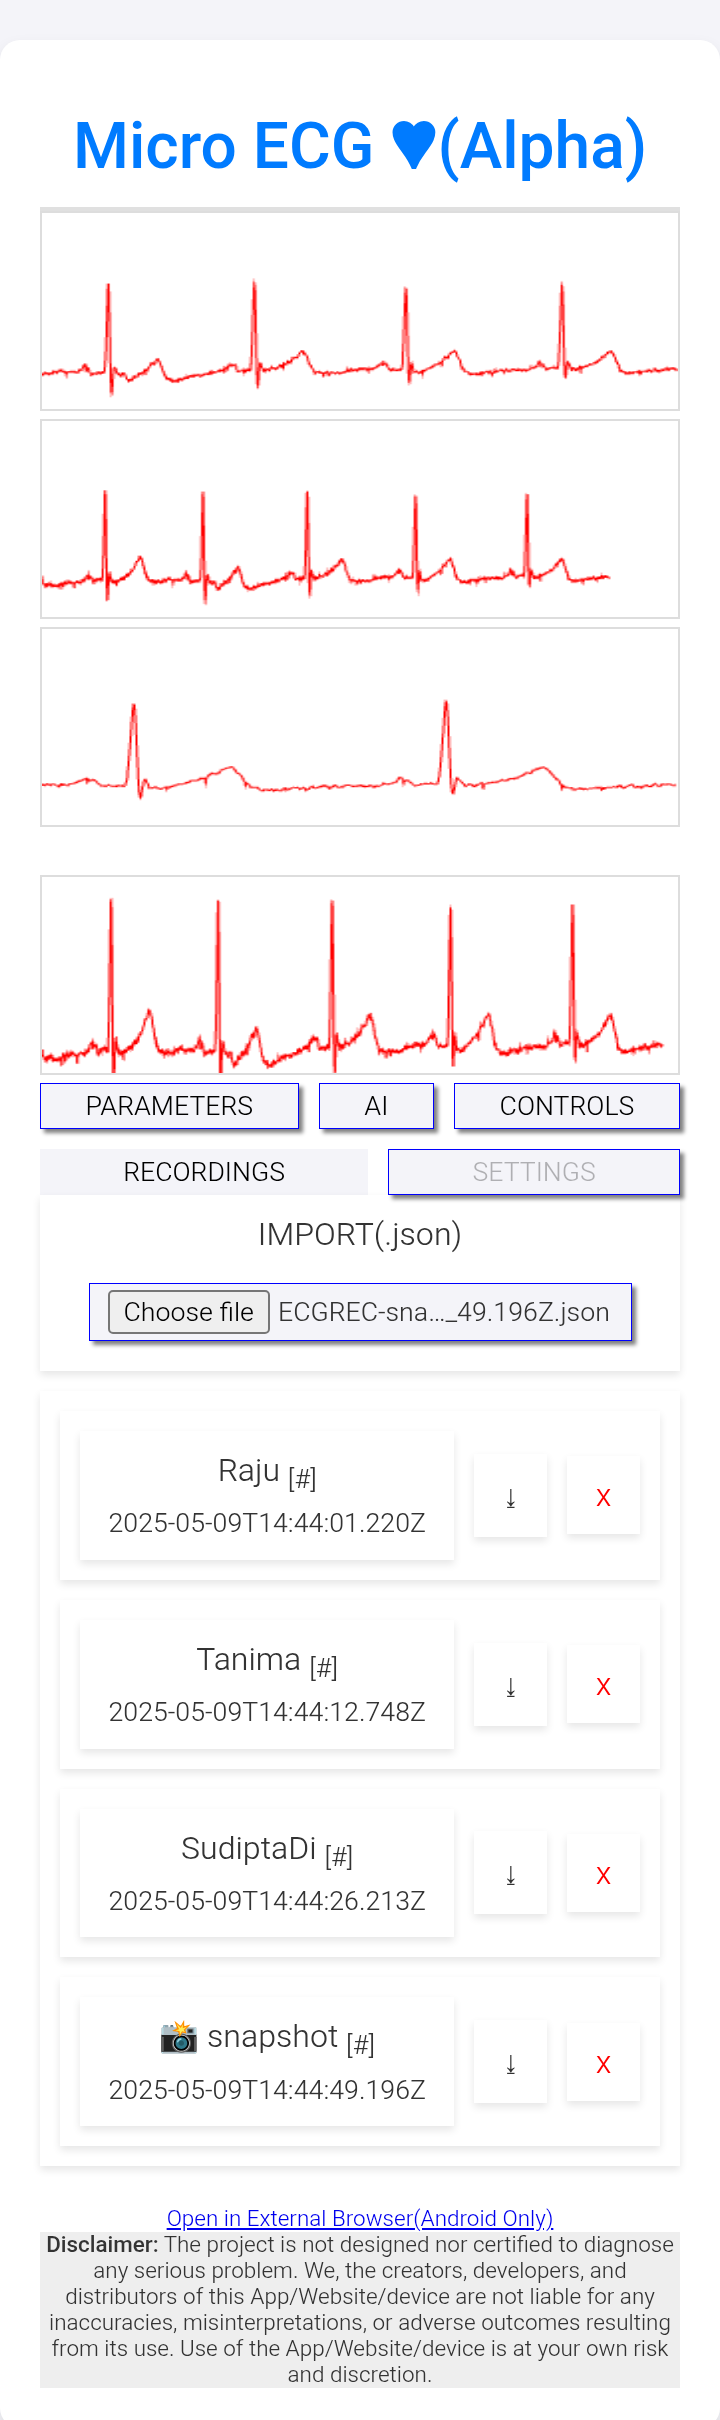
\includegraphics[width=\textwidth]{images/result-recordings.png}
        \caption{ECG signal recording/logging and snapshot}
    \end{subfigure}
    \caption{AI, recording/logging, snapshot - RESULT}
\end{figure}
% \begin{figure}[h]
%     \centering
%     % \includegraphics[width=0.75\textwidth]{images/dso_block_diagram.jpg
%     \caption{Live ECG signal rendering on browser}
% \end{figure}






\chapter{Future Scope}

\section{Multi-Lead Expansion}
The current architecture supports one lead. A future version can include:
\begin{itemize}
    \item Switchable analog multiplexers for multiple inputs.
    \item ESP32 with multiple ADCs for parallel acquisition.
    \item Software logic for lead selection and waveform labeling.
\end{itemize}

\section{AI-Assisted Diagnostics}
Currently, AI classification is supported via external APIs. Future integration may include:
\begin{itemize}
    \item On-device TinyML inference.
    \item Real-time rhythm classification (AFib, bradycardia).
    \item Training models on locally collected ECG data.
\end{itemize}

\section{Bluetooth Compatibility}
Adding BLE for optional use with mobile apps. ESP32 supports dual-mode communication.

\section{Remote Monitoring and Logging}
With internet uplink, data can be:
\begin{itemize}
    \item Stored on cloud databases.
    \item Viewed remotely by doctors via web dashboards.
    \item Annotated and replayed for longitudinal studies.
\end{itemize}

\section{Design for Mass Deployment}
\begin{itemize}
    \item Improve enclosure durability (IP-rated).
    \item Medical-grade electrode support.
    \item Certifications for clinical trials and diagnostics.
\end{itemize}




\chapter{Conclusion}

The aim of this project was to conceptualize, design, and implement a fully functional, real-time ECG monitoring system that integrates analog and digital subsystems into a single, self-contained platform. From signal acquisition to wireless visualization, the system demonstrates a complete end-to-end solution rooted in precision sensing, signal conditioning, embedded programming, and user-interface development.

Through the integration of bio-signal amplification, hardware noise filtering, ADC-based data acquisition, and WiFi-enabled microcontroller interfacing, the project showcases how complex physiological signals can be processed and presented in a low-latency digital form without relying on external computing infrastructure.

Key outcomes include:
\begin{itemize}
    \item A self-powered, embedded system for biomedical signal monitoring.
    \item Custom hardware design supporting both finger and chest electrode inputs.
    \item Real-time, browser-based UI without dependency on native applications.
    \item Use of WebSocket protocol for low-latency data transmission.
    \item Modular and extensible architecture suitable for future integration with intelligent systems.
\end{itemize}

This project not only reflects a thorough understanding of core design principles across analog, digital, and communication systems, but also translates theoretical knowledge into a practical solution with real-world applicability. The prototype validates the potential of combining circuit design, embedded control, wireless networking, and interactive interfaces in solving domain-specific challenges—making it a strong example of applied engineering for health-focused innovation.


\addcontentsline{toc}{chapter}{Annexure}
\appendix
\chapter*{\centering \large Annexure A}
\subsection*{Microcontroller program}
\begin{lstlisting}[style=htmlcssjs, language=CPP]
#include <DNSServer.h>
#include <WebSocketsServer.h>
#include <ESP8266WebServer.h>
// #include <ESP8266mDNS.h>

const byte DNS_PORT = 53;
IPAddress apIP(172, 217, 28, 1);
DNSServer dnsServer;
ESP8266WebServer server(80);
WebSocketsServer webSocket = WebSocketsServer(81);


// ADC buffer and indexing variables
int *adcBuffer = nullptr;    // Dynamic buffer pointer
int sampleIndex = 0;
int sps = 10;                // Default saadcBuffermples per second
unsigned long previousMillis = 0;
const long sendInterval = 300;   // Time interval to send data (333ms)

unsigned long lastSampleTime = 0;  // Time of last sample
long sampleInterval = 1000 / sps;  // Interval between each sample based on SPS


String webServerIndexPage = "[WEB UI CODE]";
String webServerSW = "[SERVISE WORKER JS]";

void webSocketEvent(uint8_t num, WStype_t type, uint8_t* payload, size_t length) {

    switch (type) {
        case WStype_DISCONNECTED:
        Serial.printf("[%u] Disconnected!\n", num);
        break;
        case WStype_CONNECTED:
        {
            IPAddress ip = webSocket.remoteIP(num);
            Serial.printf("[%u] Connected from %d.%d.%d.%d url: %s\n", num, ip[0], ip[1], ip[2], ip[3], payload);
        }
        break;
        case WStype_TEXT:
        Serial.printf("[%u] get Text: %s\n", num, payload);

        //int arrayLen = payload - 0;
        int newSps = atoi((const char*)payload);

        // Try to parse the samples per second (SPS) from the message
        if (newSps > 0 && newSps != sps) {
            // Adjust the number of samples per second if needed
            sps = newSps;

            // Reallocate the ADC buffer with the new size
            if (adcBuffer != nullptr) {
                free(adcBuffer); // Free old buffer
            }
            adcBuffer = (int *)malloc(sps * sizeof(int)); // Allocate new buffer

            // Update sampling interval based on SPS
            sampleInterval = 1000 / sps;

            Serial.print("New SPS: ");
            Serial.println(sps);
        }


        break;
    }
}

void handleNotFound() {
    server.sendHeader("Location", "/", true); //Redirect to our html web page
    server.send(301, "text/plane", "");
}


void setup() {
    Serial.begin(115200);

    // Serial.setDebugOutput(true);

    Serial.println();
    Serial.println();
    Serial.println();

    for (uint8_t t = 4; t > 0; t--) {
        Serial.printf("[SETUP] BOOT WAIT %d...\n", t);
        Serial.flush();
        delay(1000);
    }

    adcBuffer = (int *)malloc(sps * sizeof(int));

    WiFi.mode(WIFI_AP);
    WiFi.softAPConfig(apIP, apIP, IPAddress(255, 255, 255, 0));
    WiFi.softAP("Micro_ECG_RANMPGroupF");
    // start webSocket server
    webSocket.begin();
    webSocket.onEvent(webSocketEvent);

    // if (MDNS.begin("esp8266")) {
    //   Serial.println("MDNS responder started");
    // }
    dnsServer.start(DNS_PORT, "*", apIP);
    // handle index
    server.on("/", []() {
        server.send(200, "text/html", webServerIndexPage);
    });
    server.on("/sw.js", []() {
        server.send(200, "application/javascript", webServerSW);
    });

    server.on("/test", []() {
        server.sendHeader("Location", "https://github.io/", true);
        server.send(302, "text/plane", "Redirecting...");
    });

    server.onNotFound(handleNotFound);
    server.begin();
    
    // // Add service to MDNS
    // MDNS.addService("http", "tcp", 80);
    // MDNS.addService("ws", "tcp", 81);
    
}

unsigned long last_10sec = 0;
unsigned int counter = 0;

void loop() {
    unsigned long t = millis();
    webSocket.loop();
    dnsServer.processNextRequest();
    server.handleClient();

    // if ((t - last_10sec) > 10 * 1000) {
    //     counter++;
    //     bool ping = (counter % 2);
    //     int i = webSocket.connectedClients(ping);
    //     Serial.printf("%d Connected websocket clients ping: %d\n", i, ping);
    //     last_10sec = millis();
    // }

    // Check if it's time to sample ADC data based on SPS
    unsigned long currentMillis = millis();

    if (currentMillis - lastSampleTime >= sampleInterval) {
        // Read ADC and store it in buffer
        adcBuffer[sampleIndex] = analogRead(A0);
        sampleIndex++;
        // Reset buffer and send data every 333ms
        if (sampleIndex >= sps) {
            Serial.printf("147................................");
            sendSamplesThroughWebSocket(adcBuffer, sps);
            sampleIndex = 0; // Reset buffer index
        }

        lastSampleTime = currentMillis;
    }
    // //Send data every 333ms
    if (currentMillis - previousMillis >= sendInterval) {
        if (sampleIndex > 0) {
            sendSamplesThroughWebSocket(adcBuffer, sampleIndex);
            sampleIndex = 0; // Reset buffer index
        }
        previousMillis = currentMillis;
    }
}

// Function to send ADC samples via WebSocket
void sendSamplesThroughWebSocket(int *samples, int count) {
  // Create a buffer to hold raw data (binary format)
  uint8_t buffer[count * sizeof(int)];
  memcpy(buffer, samples, count * sizeof(int));  // Copy ADC samples to buffer

  // Send the buffer as a binary message over WebSocket
  webSocket.broadcastBIN(buffer, count * sizeof(int));
}
\end{lstlisting}














\subsection*{Web Development for UI}
\subsubsection*{HTML}
\begin{lstlisting}[style=htmlcssjs]
<!DOCTYPE html>
<html lang="en">
<head>
    <meta charset="UTF-8">
    <meta name="viewport" content="width=device-width, initial-scale=1">
    <title>Micro ECG</title>
</head>
<body>
    <noscript>
        Please Enable JavaScript in your browser...!!
    </noscript>
    <div class="container">
        <div class="header">
            <h1>Micro ECG &hearts;(Alpha)</h1>
        </div>
        <div id="snap-container" class="snap-container"></div>
        <div class="canvas-container">
            <canvas id="ecgCanvas"></canvas>
        </div>
        <div class="tabs">
            <button active data-id="parameters">PARAMETERS</button>
            <button data-id="ai-assistant">AI</button>
            <button data-id="controls">CONTROLS</button>
            <button data-id="recordings">RECORDINGS</button>
            <button data-id="settings" disabled>SETTINGS</button>
        </div>
        <div class="tab-contents">
            <div active class="parameters">
                <!-- <div class="parameter">
                    <input type="range" oninput="" value="" />
                </div> -->
                <div class="parameter">
                    <span>Result: <span id="param-result"> •_° </span> </span>
                </div>
                <div class="parameter">
                    <span>Heart Rate: <span id="param-hr"> •_° </span> bpm</span>
                </div>
                <div class="parameter">
                    <span>QRS Duration: <span id="param-qrs"> •_° </span> ms</span>
                </div>
                <div class="parameter">
                    <span>QT Interval: <span id="param-qt"> •_° </span> ms</span>
                </div>
                <div class="parameter">
                    <span>PR Interval: <span id="param-pr"> •_° </span> ms</span>
                </div>
                <div class="parameter">
                   <span> ST Interval: <span id="param-st"> •_° </span> ms </span>
                </div>
            </div>
            <div class="ai-assistant">
                <h2>AI Assistant</h2>
                <p id="ai-output"></p>
                <button id="ai-assistBtn">&#x27F3; Get Assistance</button>
            </div>
            <div class="controls">
                <div style="width:100%" class="control"></div>
                <div class="control pushButton" data-toggle="isHold">
                    <span>HOLD</span>
                </div>
                <div id="recordBtn" class="control pushButton">
                    <span>RECORD</span>
                </div>
                <div class="control" onclick="data_plot = []">
                    <span>CLEAR</span>
                </div>
                <div id="takeSnapBtn" class="control">
                    <span>SNAP</span>
                </div>
                <div style="width:100%" class="control"></div>
                <div class="control">
                    <span>TIME/DIV</span><br /> &minus; <input class="multiturn minZero" type="range" oninput="scale.x = this.dataset.value/10" min="0" max="100" data-default="50" value="50"/> &plus;
                </div>
                <div class="control">
                    <span>VOLT/DIV</span><br /> &minus; <input class="multiturn" type="range" oninput="scale.y = this.dataset.value/10" min="0" max="100" data-default="120" value="50"/> &plus;
                </div>
                <div class="control">
                    <span>POSITION VERTICAL</span><br /> &#9650; <input class="multiturn" type="range" oninput="move.y = this.dataset.value*10" min="0" max="100" data-default="13" value="50"/> &#9660;
                </div>
                <div class="control">
                    <span>POSITION HORIZONTAL</span><br /> &#9198; <input class="multiturn minZero" type="range" oninput="move.x = this.dataset.value*10" min="0" max="100" data-default="0" value="50"/> &#9197;
                </div>
                <div style="width:100%" class="control"></div>
            </div>
            <div class="flexbox recordings">
                <div style="width:100%" class="flexbox"><label for="">IMPORT(.json)</label><input id="recordingImport" type="file" accept=".json"/></div>
                <div id="recordings" class="flexbox">
                    <div class="flexbox">
                        <div class="pushButton">NO RECORD FOUND<br /><sub>mm:hh dd-mm-yyyy</sub></div>
                        <div class="download">&#x2913;</div>
                        <div class="download">x</div>
                    </div>
                </div>
            </div>
            <!-- <div class="settings">
                <div class="setting network">
                    <h2>Network</h2>
                    <h3>Available Access Points...</h3><button id="refresh-AP">Refresh</button>
                    <div id="wifi-list">
                        <div>SSID(signal) <button>Connect</button></div>
                        <div>SSID(signal) <button>Connect</button></div>
                        <div>SSID(signal) <button>Connect</button></div>
                    </div>
                    <h4>Connect to Hidden Network</h4>
                    <form id="hidden-network-form">
                      <input type="text" id="ssid" placeholder="SSID" required><br />
                      <input type="password" id="password" placeholder="Password" required><br />
                      <button type="submit">Connect</button>
                    </form>
                </div>
                <div class="setting">
                    <h2>Hardware</h2>
                    Samples Per Second: <input style="width:50px" placeholder="999" type="number"/>
                    <hr /><hr />
                    <button class="danger" style="background-color:#f005,border">Reset</button>
                </div>
            </div> -->
        </div>
        <div class="footer">
            <a href="#" onclick="window.open('/','_blank)">Open in External Browser(Android Only)</a>
            <p style="display:block;background-color:#eee;"><b>Disclaimer:</b> The project is not designed nor certified to diagnose any serious problem.
            We, the creators, developers, and distributors of this App/Website/device are not liable for any inaccuracies, misinterpretations, or adverse outcomes resulting from its use. Use of the App/Website/device is at your own risk and discretion.</p>
        </div>
    </div>
</body>
</html>
\end{lstlisting}





\subsubsection*{CSS}
\begin{lstlisting}[style=htmlcssjs]
* {
    margin: 0;
    padding: 0;
    box-sizing: border-box;
    font-family: Arial, sans-serif;
}
body {
    background: #f4f4f9;
    color: #333;
}
button , input{
    padding: 3px 9px;
    margin: 5px;
    background-color: #f4f4f9;
    border: 0.1px solid #00f;
    box-shadow: 2px 2px 2px gray;
}
button:hover , input:hover{
   box-shadow: none;
}
.pushButton[active]{
    background-color: #0f05;
}
.container {
    max-width: 1200px;
    margin: 20px auto;
    padding: 20px;
    background: #fff;
    border-radius: 10px;
    box-shadow: 0 4px 8px rgba(0, 0, 0, 0.1);
}
.header {
    text-align: center;
    padding: 10px 0;
    border-bottom: 2px solid #e0e0e0;
}
.header h1 {
    font-size: 2rem;
    color: #007bff;
}
.snap-container{
    width: 100%;
    margin: auto;
}
.canvas-container {
    margin-top: 20px;
    text-align: center;
    position: sticky; 
    top: 0px;
    pointer-events: none;
    background-color: #fff5;
}
canvas, .snap-container img {
    border: 1px solid #ddd;
    width: 100%;
    height: 100px;
}
.tabs{
    display: flex;
    flex-wrap: wrap;
    gap: 10px;
}
.tabs button {
    margin: 0px;
    flex: 1 1 auto;
}
.tabs button[active] {
    box-shadow: none;
    border: none;
}
.tab-contents>div:not([active]) {
    display: none;
}
.parameters {
    display: flex;
    flex-wrap: wrap;
    gap: 20px;
    padding: 20px 0;
}
.parameter {
    flex: 1 1 auto;
    background: #f9f9f9;
    padding: 10px;
    border-radius: 5px;
    box-shadow: 0 2px 4px rgba(0, 0, 0, 0.1);
    text-align: center;
    min-width: 30%;
}
.parameter span {
    font-size: 1rem;
    color: #555;
    font-weight: bold;
    white-space: nowrap;
}
.controls , .settings, .flexbox{
    display: flex;
    flex-wrap: wrap;
    justify-content: center;
    align-items: center;
    gap: 10px;
}
.control , .flexbox div, .setting{
    flex: 1 1 auto;
    text-align: center;
    padding: 10px;
    box-shadow: 0 2px 4px rgba(0, 0, 0, 0.1);
}
.ai-assistant {
    margin: 20px 0;
    background: #e7f5ff;
    padding: 15px;
    border-radius: 8px;
    text-align: center;
    box-shadow: 0 2px 4px rgba(0, 0, 0, 0.1);
}
.ai-assistant h2 {
    font-size: 1.5rem;
    color: #00f;
}
.ai-assistant p {
    font-size: 1rem;
    color: #444;
    margin-top: 10px;
}
.footer {
    text-align: center;
    margin-top: 20px;
    font-size: 0.7rem;
    color: #333;
}
.danger {
    color: red!important;
    border-color: red!important;
}
@media (max-width: 668px) {
    .parameters {
        flex-direction: column;
    }
    .flexbox{
        width: 100%;
    }
}
\end{lstlisting}




\subsubsection*{JavaScript}
\begin{lstlisting}[style=htmlcssjs]
//var data_plot = [0,1200,0,1200,0,1200];
var data_plot = new Array(200).fill(3300);
//var data_plot = new Array(200).fill(1600);

// --- HELPERS --- //
document.querySelectorAll(".pushButton").forEach(o => {
    o.addEventListener('click', (e) => {
        o.hasAttribute('active') ? o.removeAttribute('active'):o.setAttribute('active','');
        window[o.dataset.toggle] = o.hasAttribute('active');
        //window[o.dataset.toggle] || e.stopPropagation();
    },true)
});

document.querySelectorAll('.multiturn').forEach(o=> {
    let disp = Number(o.dataset.default);
    const max = Number(o.max);
    const min = Number(o.min);

    o.addEventListener('change', () => {
        if (o.value <= min && !(o.classList.contains('minZero') && disp <= 0)) {
            o.value = max/2;
            disp -= max/2
        }
        if (o.value >= max) {
            o.value = max/2;
            disp += max/2
        }
    });
    o.addEventListener('input', () => {
        if(o.classList.contains('minZero') && disp + Number(o.value-(max/2))  <= 0) return 0;
        o.dataset.value = disp + Number(o.value-(max/2));
    });
});

// ---- Custom alert and prompt ----//
(() => {
  const a = document.createElement("div");
  a.style = "position:fixed;top:0;left:0;width:100%;height:100%;background:#0005;display:flex;justify-content:center;align-items:center;visibility:hidden;z-index:1000;";

  const b = document.createElement("div");
  b.style = "background:white;padding:20px;border-radius:5px;text-align:center;box-shadow:0 2px 5px rgba(0,0,0,0.3);width:250px;";

  const c = document.createElement("p");
  const d = document.createElement("input");
  d.type = "text";
  d.style = "display:none;margin-bottom:15px;padding:5px;width:100%;";

  const e = document.createElement("button");
  e.textContent = "OK";
  e.style = "background:#007bff;color:white;";

  const f = document.createElement("button");
  f.textContent = "Cancel";
  f.style = "background:#dc3545;color:white;display:none;";

  b.append(c, d, e, f);
  a.appendChild(b);
  document.body.appendChild(a);

  window.alert = msg => { c.textContent = msg; d.style.display = "none"; f.style.display = "none"; e.onclick = () => a.style.visibility = "hidden"; a.style.visibility = "visible"; };
  window.prompt = (msg, cb=(o=>{return false}),cc=(o=>{return false})) => { c.textContent = msg; d.style.display = "block"; f.style.display = "inline-block"; d.value = ""; e.onclick = () => { a.style.visibility = "hidden"; cb(d.value); }; f.onclick = () => {a.style.visibility = "hidden";cc(); }; a.style.visibility = "visible"; };
})();

// ---- Custom Notification ----//
(() => {
    document.head.appendChild(Object.assign(document.createElement('style'), { innerHTML: `
        .notify-container {
            width: 100%; max-height: 230px; overflow: scroll; display: flex; flex-direction: column;
            align-items: center; position: fixed; top: 10px; left: 0; pointer-events: none;
        }
        .notify-container > div {
            max-width: 400px; margin: 10px; border-radius: 5px; text-align: center; padding: 10px 20px;
            background: #eef; color: #00f; position: relative; box-shadow: 0 2px 5px rgba(0, 0, 0, 0.2);
            transition: transform 0.5s; pointer-events: auto;
        }
        .notify-container > div:hover { transform: translateY(10%); }
        .notifyClose { position: absolute; right: 5px; bottom: 25%; font-weight: bold; cursor: pointer; }
    `}));

    let container = document.body.appendChild(Object.assign(document.createElement('div'), { className: "notify-container" }));

    document.notify = (t = '', c, s) => {
        let div = Object.assign(document.createElement('div'), { innerText: t });
        div.appendChild(Object.assign(document.createElement('div'), { className: "notifyClose", innerText: "×", onclick: () => div.remove() }));
        div.style = { error: 'background:#fdd;color:#f00;', warning: 'background:#ffc;color:#f00;', success: 'background:#cfc;color:#080;' }[c] || '';
        setTimeout(() => div.remove(), s || (container.innerText.length + t.length) * 200);
        container.appendChild(div);
    };
})();


var recordingQue = {
    count:0,
    data:[]
}
async function feedData(arr) {
    //let sps = 333;
    //let i = 0, t = await setInterval(() => (i < arr.length && !isHold) ? data_plot.push(arr[i++]) : clearInterval(t), 1000 / sps);

    isHold || data_plot.push(...arr)
    if(isRecording){
        recordingQue.data.push(...arr);
        recordingQue.count++;
        if(!(recordingQue.count%10)){
            logData(recordingQue.data);
            recordingQue.data = [];
        }
    }
}







const wSocket = new WebSocket('ws://172.217.28.1:81');
//const wSocket = new WebSocket('ws://'+location.hostname+':81');
wSocket.binaryType = 'arraybuffer';
wSocket.onopen = function() {
    document.notify('WebSocket: Connection established!', 'success'); wSocket.send(300);
};
wSocket.onmessage = function(event) {
    const data = new Uint16Array(event.data);
    let adcValues = [];
    for (let i = 0; i < data.length; i += 2) {
        let value = data[i] | (data[i + 1] << 8);
        adcValues.push((value*1.4)+1600);
    }
    feedData(adcValues,300);
};
wSocket.onerror = function(error) {
    document.notify('WebSocket: Error ' + error, 'error');
};
wSocket.onclose = function() {
    document.notify('WebSocket: Connection closed', 'warning');
}; 
//setInterval(() => feedData(new Array(100).fill(1840)) ,1000)
//setInterval(() => feedData([Math.random()*3000,Math.random()*3000,Math.random()*3000,Math.random()*3000,Math.random()*3000,Math.random()*3000,Math.random()*3000,Math.random()*3000,Math.random()*3000,Math.random()*3000,Math.random()*3000,Math.random()*3000,Math.random()*3000,Math.random()*3000,Math.random()*3000,80]) ,300)



// ---- Init ----//
var graphCanvas = document.getElementById("ecgCanvas");
var ctx = graphCanvas.getContext('2d');
var scale = {x:5,y:12};//y:8.6
var move = {x:0,y:130};//y:0
var isHold = false;
var isRecording = false;
var recording = [];
var ECGResult = [];

// ---- Responsive Canvas ----//
graphCanvas.width = graphCanvas.offsetParent.offsetWidth;
addEventListener('resize', () => {
    graphCanvas.width = graphCanvas.offsetParent.offsetWidth;
})


// ---- service worker ----//
if ("serviceWorker" in navigator) {
    navigator.serviceWorker.register("./sw.js").catch(console.log);
}

// ---- Plot Graph ----//
function render() {
    ctx.clearRect(0, 0, graphCanvas.width, graphCanvas.height);
    
    
    // virtualCanvas
    var VC = data_plot.slice(-graphCanvas.width*scale.x-move.x,-1-move.x);
    VC = VC.map(o => {
        return o/scale.y-move.y
    });
    
    ECGResult = ECGinterpreter(VC,500);
    
    ctx.beginPath();
    ctx.moveTo(...OLB(0, VC[0]));
    
    for(var i=0; i < VC.length;i++){
       ctx.lineTo(...OLB(i/scale.x, VC[i]));
    }
    ctx.strokeStyle = "red";
    ctx.stroke();
    
    function OLB(x , y) {
        // origin Left - Bottom
        return [x , graphCanvas.height-y];
    }
    
   requestAnimationFrame(render);
}
setTimeout(render,100);



// --- NEVIGATION - TABS --- //
(() => {
const tabs = document.querySelectorAll('.tabs>button');
const contents = document.querySelectorAll('.tab-contents>div');

tabs.forEach(tab => {
  tab.addEventListener('click', () => {
    tabs.forEach(t => t.removeAttribute('active'));
    contents.forEach(c => c.removeAttribute('active'));
    tab.setAttribute('active','');
    document.querySelector('.' + tab.dataset.id).setAttribute('active','');
})})
})();



document.getElementById("takeSnapBtn").addEventListener('click',()=>{
    const img = document.createElement('img');
    img.src = graphCanvas.toDataURL("image/png");
    img.addEventListener('click',img.remove);
    document.getElementById("snap-container").appendChild(img);
    prompt("Save SNAPSHOT As:",(name)=>{
    dbManager.add('metadata',
    {
        name: name || "SNAPSHOT",
        startTime: new Date().toISOString(),
        snapURL: img.src,
        type: "snapshot"
    })})
});



// ---- IndexedDB Manager ----//
class IDBManager {
    constructor({
        dbName, dbVersion, onUpgrade
    }) {
        this.dbName = dbName;
        this.dbVersion = dbVersion;
        this.onUpgrade = onUpgrade;
        this.db = null;
        this.changeEventListeners = [];
    }

    open() {
        if (this.db) return Promise.resolve(this.db);

        return new Promise((resolve, reject) => {
            const request = indexedDB.open(this.dbName, this.dbVersion);

            request.onerror = () => reject(request.error);
            request.onblocked = () => reject(new Error('Database upgrade blocked'));

            request.onsuccess = (event) => {
                this.db = event.target.result;
                resolve(this.db);
            };

            request.onupgradeneeded = (event) => {
                this.db = event.target.result;
                if (typeof this.onUpgrade === 'function') {
                    this.onUpgrade(
                        this.db,
                        event.oldVersion,
                        event.newVersion,
                        event.target.transaction
                    );
                }
            };
        });
    }

    async add(storeName, item) {
        await this.open();
        this.changeEventListener(storeName);
        return this._executeTransaction(storeName,
            'readwrite',
            (store) => {
                return store.add(item);
        });
    }

    async get(storeName, id) {
        await this.open();
        return this._executeTransaction(storeName,
            'readonly',
            (store) => {
                return store.get(id);
        });
    }

    async update(storeName, id, updates) {
        await this.open();
        this.changeEventListener(storeName);
        return this._executeTransaction(storeName,
            'readwrite',
            async (store) => {
                const request = await store.get(id);
                request.onsuccess = o => {
                    var item = o.target.result;
                    Object.assign(item, updates);
                    store.put(item);
                }
        });
    }

    async delete(storeName, id) {
        await this.open();
        this.changeEventListener(storeName);
        return this._executeTransaction(storeName,
            'readwrite',
            (store) => {
                return store.delete(id);
        });
    }

    async getAll(storeName) {
        await this.open();
        return this._executeTransaction(storeName,
            'readonly',
            (store) => {
                return store.getAll();
            });
    }

    async clear(storeName) {
        await this.open();
        this.changeEventListener(storeName);
        return this._executeTransaction(storeName,
            'readwrite',
            (store) => {
                return store.clear();
        });
    }
    changeEventListener(storeName) {
        this.changeEventListeners.forEach(o => o.storeName == storeName && o.action());
    }
    addChangeEventListener(o,sn) {
        this.changeEventListeners.push({
            action : o,
            storeName: sn
        });
    }
    async _executeTransaction(storeName, mode, operation) {
        return new Promise((resolve, reject) => {
            const transaction = this.db.transaction(storeName, mode);
            const store = transaction.objectStore(storeName);

            const request = operation(store);
            request.onerror = () => reject(request.error);

            transaction.oncomplete = (e) => {
                resolve(request.result);
            };
            transaction.onerror = () => reject(transaction.error);
        });
    }

    close() {
        if (this.db) {
            this.db.close();
            this.db = null;
        }
    }
}



// ---- Manage Recording ----//
const dbManager = new IDBManager({
    dbName: 'EcgRecordings',
    dbVersion: 1,
    onUpgrade: (db, oldVersion, newVersion, transaction) => {
        if (!db.objectStoreNames.contains('metadata')) {
            const store = db.createObjectStore('metadata', {
                keyPath: 'id', autoIncrement: true
            });
        }

        if (!db.objectStoreNames.contains('dataChunks')) {
            const store = db.createObjectStore('dataChunks', {
                keyPath: 'id', autoIncrement: true
            });
        }
    }
});

var dbVariables = {
    chunkNo: 0,
    metadataID: null,
    prevChunkID: null
};

async function startRecording(name) {
    dbVariables.metadataID = await dbManager.add('metadata',
        {
            name: name || "RECORD",
            startTime: new Date().toISOString(),
            endTime: null,
            dataChunkId: null,
            type: "dataStream"
        });
    dbVariables.chunkNo = 0;
    dbVariables.prevChunkID = null;
    isRecording = true
}

async function logData(data) {
    dbVariables.chunkNo++;
    var currChunkID = await dbManager.add('dataChunks',
        {
            data: data,
            chunkNo: dbVariables.chunkNo
        });
    if (dbVariables.chunkNo == 1) {
        await dbManager.update('metadata', dbVariables.metadataID, {
            dataChunkId: currChunkID
        });
    } else {
        await dbManager.update('dataChunks', dbVariables.prevChunkID, {
            nextChunkId: currChunkID
        });
    }
    await dbManager.update('metadata', dbVariables.metadataID, {
        totalChunks: dbVariables.chunkNo,
        endTime: new Date().toISOString()
    })
    dbVariables.prevChunkID = currChunkID;
}

document.getElementById("recordBtn").addEventListener('click',(e) => {
    const recordBtn = e.currentTarget;
    isRecording = false
    if(recordBtn.hasAttribute("active")){
        prompt("Save RECORDING As:",startRecording,() => recordBtn.removeAttribute("active"));
    }
})


//dbManager.getAll('metadata').then(console.log)
//dbManager.getAll('dataChunks').then(console.log)


async function updateRecordingUI() {
    const metadata = await dbManager.getAll("metadata");
    const recordingsDIV = document.getElementById("recordings");
    recordingsDIV.innerText = metadata.length ? '':'NO DATA FOUND!!';
    metadata.forEach((o) => {
        const flexBox = document.createElement("div");
        flexBox.className = "flexbox";
        
        const viewBtn = document.createElement("div");
        viewBtn.innerHTML = `${o.type == "snapshot"?'&#128248;':''} ${o.name} <sub> [${o.totalChunks || '#'}]</sub> <br /><sub>${o.startTime}</sub>`; 
        viewBtn.addEventListener('click',async (e) => {
            if(o.type == "snapshot"){
                const img = document.createElement('img');
                img.src = o.snapURL;
                img.addEventListener('click',img.remove);
                document.getElementById("snap-container").appendChild(img);
            }
            if(o.type == "dataStream"){
                isHold = true;
                data_plot = [];
                let nextChunkID = o.dataChunkId;
                while (nextChunkID) {
                    const chunk = await dbManager.get("dataChunks", nextChunkID);
                    if (!chunk) break;
                    data_plot.push(...chunk.data);
                    nextChunkID = chunk.nextChunkId || null;
                }
            }
        })
        
        const delBtn = document.createElement("div");
        delBtn.className = "danger";
        delBtn.innerHTML = "x";
        delBtn.addEventListener('click', async () => {
            if(isRecording) {
                //prevent delete while recording
                document.notify("can't delete while recording!!","error")
                return false;
            }
            
            dbManager.delete("metadata",o.id);
            
            let nextChunkID = o.dataChunkId;
            while (nextChunkID) {
                const chunk = await dbManager.get("dataChunks", nextChunkID);
                if (!chunk) break;
                dbManager.delete("dataChunks",nextChunkID);
                nextChunkID = chunk.nextChunkId || null;
            }
        })
        
        const downloadBtn = document.createElement("div");
        downloadBtn.innerHTML = "&#x2913;";
        downloadBtn.addEventListener('click',() => {
            exportData(o.id);
        })
        
        flexBox.appendChild(viewBtn);
        flexBox.appendChild(downloadBtn);
        flexBox.appendChild(delBtn);
        recordingsDIV.appendChild(flexBox);
    })
}
updateRecordingUI();
dbManager.addChangeEventListener(updateRecordingUI,"metadata");
async function exportData(id) {
    const metadata = await dbManager.get("metadata", id);

    let chunks = [], nextChunkID = metadata.dataChunkId;
    while (nextChunkID) {
        const chunk = await dbManager.get("dataChunks", nextChunkID);
        if (!chunk) break;
        chunks.length > 0?chunks[0].data.push(...chunk.data):chunks.push(chunk);
        nextChunkID = chunk.nextChunkId || null;
    }
    
    if(nextChunkID){
        metadata.totalChunks = 1;
        delete chunks[0].nextChunkId;
    }

    const blob = new Blob([JSON.stringify({ metadata, chunks })], { type: "application/json" });
    const a = Object.assign(document.createElement('a'), { href: URL.createObjectURL(blob), download: "ECGREC-"+metadata.name+metadata.startTime+".json" });
    a.click();
}

document.getElementById('recordingImport').addEventListener('change', async event => {
    const reader = new FileReader();
    reader.onload = async e => {
        const { metadata, chunks } = JSON.parse(e.target.result);
        delete metadata.id;
        
        if(metadata.dataChunkId){
            var chunk = chunks.find(o => o.id == metadata.dataChunkId);
            delete chunk.id;
            metadata.dataChunkId = await dbManager.add("dataChunks", chunk);
        }
        await dbManager.add("metadata", metadata);
    };
    reader.readAsText(event.target.files[0])
});



var ECGinterpreter = (function (ecgSamples,sampleRate) {
var result = {
    min: Math.min(...ecgSamples),
    max: Math.max(...ecgSamples),
    sps : sampleRate,
    hr: [],
    R: [],
    PQ: [],
    QR: [],
    RS: [],
    ST: []
};

// ---- Find R peaks --- //
result.R = (input => {
    const min = result.min, mid = (result.max - min) * 0.8;
    let peaks = [], max = -Infinity, idx = -1;
    
    for (let i in input) {
        if (input[i] > min + mid) {
            if (input[i] > max) {
                max = input[i];
                idx = i;
            }
        } else if (idx !== -1) {
            peaks.push(Number(idx));
            max = -Infinity;
            idx = -1;
        }
    }
    if (idx !== -1) peaks.push(Number(idx));
    return peaks;
})(ecgSamples);


// ---- Calculate Heart Rate --- //
result.hr = Math.round(((result.R.length-1)*sampleRate*60)/(result.R.at(-1) - result.R[0]));

// ---- Find PQST peaks --- //
for(var i = 0; i < result.R.length-1;i++){
    var rrChunk = ecgSamples.slice(result.R[i],result.R[i+1]);
    var RS = rrChunk.indexOf(Math.min(...rrChunk));
    result.RS.push(RS);
    
    var srHalfChunk = rrChunk.slice(RS,RS+(rrChunk.length/2));
    var ST = srHalfChunk.indexOf(Math.max(...srHalfChunk));
    result.ST.push(ST);
    
    var srHalfChunk2 = rrChunk.slice(RS+(rrChunk.length/2),-1);
    var QR = 0;
    for(let k = srHalfChunk2.length - 1; k >= 0 && srHalfChunk2.at(k)-srHalfChunk2.at(k-1) >= 0; k--) QR = srHalfChunk2.length-k ;
    result.QR.push(QR);
    
    var sqHalfChunk2 = srHalfChunk2.slice(0,-QR);
    var PQ = sqHalfChunk2.length-sqHalfChunk2.indexOf(Math.max(...sqHalfChunk2));
    result.PQ.push(PQ);
}
//data_plot = rrChunk;
/*data_plot[data_plot.length-QR] = 2999;
data_plot[data_plot.length-PQ-QR] = 2999;
data_plot[RS] = 2999;
data_plot[RS+ST] = 2999;*/


function analyzeECG(result) {
  if (result.hr < 5) {
    return "Rest In Peace 🕊️";
  }
  if (result.hr < 60) {
    return "Abnormal: Bradycardia";
  }
  if (result.hr > 300) {
    return "Invalid Data...!!";
  }
  if (result.hr > 100) {
    return "Abnormal: Tachycardia";
  }
  return "Normal ECG";
}



// ---- Update UI --- //
(eles => {
    for(var i in eles){document.querySelector(i).innerText = (typeof eles[i] == 'number'?Math.round(eles[i]):eles[i]) || "•_°"
}})
({
    "#param-result": analyzeECG(result),
    "#param-hr": result.hr,
    "#param-qrs": (result.QR[0] + result.RS[0])*1e3/sampleRate,
    "#param-qt": (result.QR[0] + result.RS[0] + result.ST[0])*1e3/sampleRate,
    "#param-pr": (result.PQ[0] + result.QR[0])*1e3/sampleRate,
    "#param-st": (result.ST[0])*1e3/sampleRate,
});

return result;
});
//let rslt = ECGinterpreter(data_plot,500);
//console.log(JSON.stringify(rslt));



// ---- Ai Assistant ----//
(() => {
var isBotAlive = false;
const botUserKey = "xxxxx.xxxxx.xxxxxx.xxxxxxx";
const botUserId = "user_xxxxxxxxxxxxxxx";
const botURL = "https://chat.botpress.cloud/xxxxxxxxxxxx-xxxxxxxxx-xxxxx";
const output = document.getElementById("ai-output");
const requestHeader = {
    accept: 'application/json',
    'x-user-key': botUserKey,
    'content-type': 'application/json'
  };

fetch(botURL+'/conversations/'+botUserId, {
  method: 'DELETE',
  headers: requestHeader
}).then(res => {
    fetch(botURL+'/conversations/get-or-create', {
      method: 'POST',
      headers: requestHeader,
      body: JSON.stringify({id: botUserId})
    }).catch(err => console.error(err));
  })
  .catch(err => console.error(err));




document.getElementById("ai-assistBtn").addEventListener('click',async () => {
    output.innerText = "In progress...!!";
    var prompt = ECGResult.hr > 300?"Invalid data!!":`User's heart rate is ${ECGResult.hr} BPM. Detected ECG :
    P-Q duration = ${ECGResult.PQ[0] * 1000 / ECGResult.sps} ms
    Q-R duration = ${ECGResult.QR[0] * 1000 / ECGResult.sps} ms
    R-S duration = ${ECGResult.RS[0] * 1000 / ECGResult.sps} ms
    S-T duration = ${ECGResult.ST[0] * 1000 / ECGResult.sps} ms
    `;

    await fetch(botURL+'/messages', {
      method: 'POST',
      headers: requestHeader,
      body: JSON.stringify({
        payload: {type: 'text', text: prompt},
        conversationId: botUserId
      })
    }).catch(err => [document.notify("Failed to connect AI Assistant...!!","error"),output.innerText = "NO Internet Connection!!"]);
    isBotAlive || startAIListening();
});
async function startAIListening() {
try {
    isBotAlive = true;
    const response = await fetch(botURL+"/conversations/"+botUserId+"/listen", {
      method: 'GET',
      headers: requestHeader
    });
    const reader = response.body.getReader();
    const decoder = new TextDecoder();
    while (true) {
        const { value, done } = await reader.read();
        if (done) break;
        decoder.decode(value)?.match(/\{.*\}/)?.forEach(o => {
        const data = JSON.parse(o).data;
        if(data && data.payload.text){
            data.isBot && (output.innerHTML = data.payload.text.replace(/\*\*(.*?)\*\*/g, "<b>$1</b>"));
        }})
    }
} catch (e) {
    isBotAlive = false;
    document.notify("AI Assistant is not responding...!!","error")
}};
})();
\end{lstlisting}



\addcontentsline{toc}{chapter}{References}
\newgeometry{top=0mm}

\begin{thebibliography}{9}
\bibitem{Parker2019}
Parker, J. (2019). \textit{Introduction to Bioinstrumentation: Fundamentals and Applications}. Pearson Education.

\bibitem{AD8232}
Analog Devices. (2014). \textit{AD8232 Data Sheet}. Retrieved from \url{https://www.analog.com/media/en/technical-documentation/data-sheets/AD8232.pdf}

\bibitem{Arias2016}
Arias, R. A., \& Llamas, J. S. (2016). Portable Electrocardiogram (ECG) for Remote Health Monitoring. \textit{Journal of Medical Systems}, 40(12), 271-285. \url{https://doi.org/10.1007/s10916-016-0620-9}

\bibitem{Espressif2015}
Espressif Systems. (2015). \textit{ESP8266EX Datasheet}. Retrieved from \url{https://www.espressif.com/sites/default/files/documentation/0a-esp8266ex_datasheet_en.pdf}

\bibitem{Kiani2018}
Kiani, M. (2018). ECG Signal Processing, Classification, and Interpretation: A Comprehensive Review. \textit{Computers in Biology and Medicine}, 59, 125-141. \url{https://doi.org/10.1016/j.compbiomed.2015.11.002}

\bibitem{Wang2017}
Wang, J., \& Xu, X. (2017). Design and Implementation of Wireless ECG Monitoring System Based on Wi-Fi. \textit{Journal of Medical Engineering \& Technology}, 41(4), 239-244. \url{https://doi.org/10.1080/03091902.2017.1362821}

\bibitem{WebSocketAPI2024}
Mozilla Developer Network. (2024). \textit{WebSocket API}. Retrieved from \url{https://developer.mozilla.org/en-US/docs/Web/API/WebSocket}

\bibitem{Tayal2018}
Tayal, A., \& Soni, R. (2018). Signal Filtering and Noise Reduction in ECG Systems: A Comparative Study. \textit{Bioengineering}, 5(4), 88-98. \url{https://doi.org/10.3390/bioengineering5040088}

\bibitem{Arduino2023}
Arduino. (2023). \textit{Arduino IDE: Integrated Development Environment}. Retrieved from \url{https://www.arduino.cc/en/software}

\end{thebibliography}

% \chapter*{\centering \large PAPER ACCEPTANCE PROOF\markboth{PAPER ACCEPTANCE PROOF}{PAPER ACCEPTANCE PROOF}}


% \chapter*{\centering \large REGISTRATION PROOF\markboth{REGISTRATION PROOF}{REGISTRATION PROOF}}


% \chapter*{\centering \large SCOPUS INDEXED CONFERENCE PROOF\markboth{SCOPUS INDEXED CONFERENCE PROOF}{SCOPUS INDEXED CONFERENCE PROOF}}


\end{document}

